

\documentclass{article}

\usepackage{tikz}

%Various Informations
\title{Call of the Wintermoon}
\author{Kaylen Wheeler \and Arvand Dorgoly}

\begin{document}

%Title
\maketitle

%The version history table
\begin{tabular}{| c | c | c | c |}
\multicolumn{4}{ l }{Version History}\\
\hline

%Title
Version Number & Edited By & Date & Comments \\ \hline

%Content
0-1 & Kaylen & 21/02/2012 & Created document\\ \hline
0-2 & Kaylen & 24/02/2012 & Started Game Overview and Game Objects and Logic sections\\ \hline

\end{tabular}

\tableofcontents

\section{Game Overview}

\subsection{Game Summary}
Play as the greatest black metal fanboy that has ever lived!  Dig your way to the bottom of the cursed glacier to obtain the Blackblood Axe, the most brutal instrument of terror ever created, to begin your worldwide reign of darkness and evil.  What evils await within, and will you be evil enough to overcome them?

\subsection{Platform}
The primary target platform will be the PC.  Development for the PC has few barriesr compared to other platforms.  Additionally, the game will be developed with relatively low technical requirements in mind, and this will open up the market to a greater number of devices.  many people own PC's, and developing for this platform will make the game very widely available.

Because this game is built with the Unity engine, further platforms, such as Xbox Live Arcade or Playstation Network may be considered at a later date, as the engine allows games to be easily ported to many platforms.

\section{Development Overview}

\subsection{Development Team}

\subsection{Development Environment}

\subsubsection{Development Hardware}

\subsubsection{Development Software}

\subsubsection{External Code}

\section{Game mechanics}

\subsection{Main Technical Requirements}

\subsection{Architecture}

Since the Unity engine is being used to create and run this game, software architecture is heavily influenced by the architecture of the engine.  However, there are still some important aspects of software architecture that must be decided on a per-game basis.  This section will outline both Unity's software architecture and how we used that architecture to implement that of our own game.

\subsubsection{Overview of Unity}

Unity is an integrated authoring tool used for creating 3D games.  By default, it provides many of the common technical elements present in most 3D games, such as high-performance graphics and physics.  Graphics are implemented using either Direct3D or OpenGL, and Unity also supports Nvidia's PhysX engine.  Implementation of each of these systems varies depending on the platform of deployment.

While the core of the engine has varying native implementations on different devices, scripting is implemented using Mono, the open-source implementation of the .NET Framework (originally created by Microsoft).  Mono provides a software framework that allows code to run on multiple platforms.  Code is compiled to the Common Language Runtime (CLR) so that code written in different high-level languages can interoperated.  In Unity, three different languages are supported - UnityScript(Similar to JavaScript), Boo (Similar to Python) and C\#.  Because of the development team's experience, C\# was chosen as the primary scripting language.

To implement scripted behaviour, the MonoBehaviour class is used.  This class is part of the UnityEngine library.  Multiple MonoBehavour objects can be attached to any game object, and each of them adds some behaviour to that object.  The class provides several hook methods, most important of which is Update, which is called once per engine update cycle (Update cycles vary, but occur approximately 60 times per second).  In addition to update functions, several event-handling functions are also provided, which can be used to detect collisions or other unexpected events that may affect the object.

\subsubsection{Our Architecture}

Using the architecture already created by Unity, our own architecture will be created to suit the purposes of our game.  The primary goals of this will be to handle the enemy AI and the combat system, which are specific to this game.

The classes involved in AI control of game entities are derived from the EntityControl class, which is itself derived from MonoBehaviour.  See Fig \ref{AI_Combat} for a UML diagram depicting EntityControl and other classes.  EntityControl's structure is based on that of a Finite State Machine.  Each instance of EntityControl contains an array of Action objects which can be indexed by any member of the EntityState enumeration.  Action is a C\# delegate type (similar to a function pointer) representing a void function with no parameters.

During the Start function (a function of MonoBehaviour that is run when a game object is initialized), the StateFunctions array is automatically initialized to default values.  During this stage, some indices of the array are matched up with their default functions (those marked as "State Function" in the UML diagram).  These functions represent states that tend to be universal across all entities.  Some indices of the array correspond to more specific states, and are therefore not initialized.  This is done so that exceptions will be thrown for invalid states, allowing bugs in code to be caught more effectively.

\begin{figure}[h!]

% Graphic for TeX using PGF
% Title: C:\Users\Kaylen\CotWM\Doc\UML\AI_Combat.dia
% Creator: Dia v0.97.1
% CreationDate: Sun Mar 11 15:41:22 2012
% For: Kaylen
% \usepackage{tikz}
% The following commands are not supported in PSTricks at present
% We define them conditionally, so when they are implemented,
% this pgf file will use them.
\ifx\du\undefined
  \newlength{\du}
\fi
\setlength{\du}{15\unitlength}
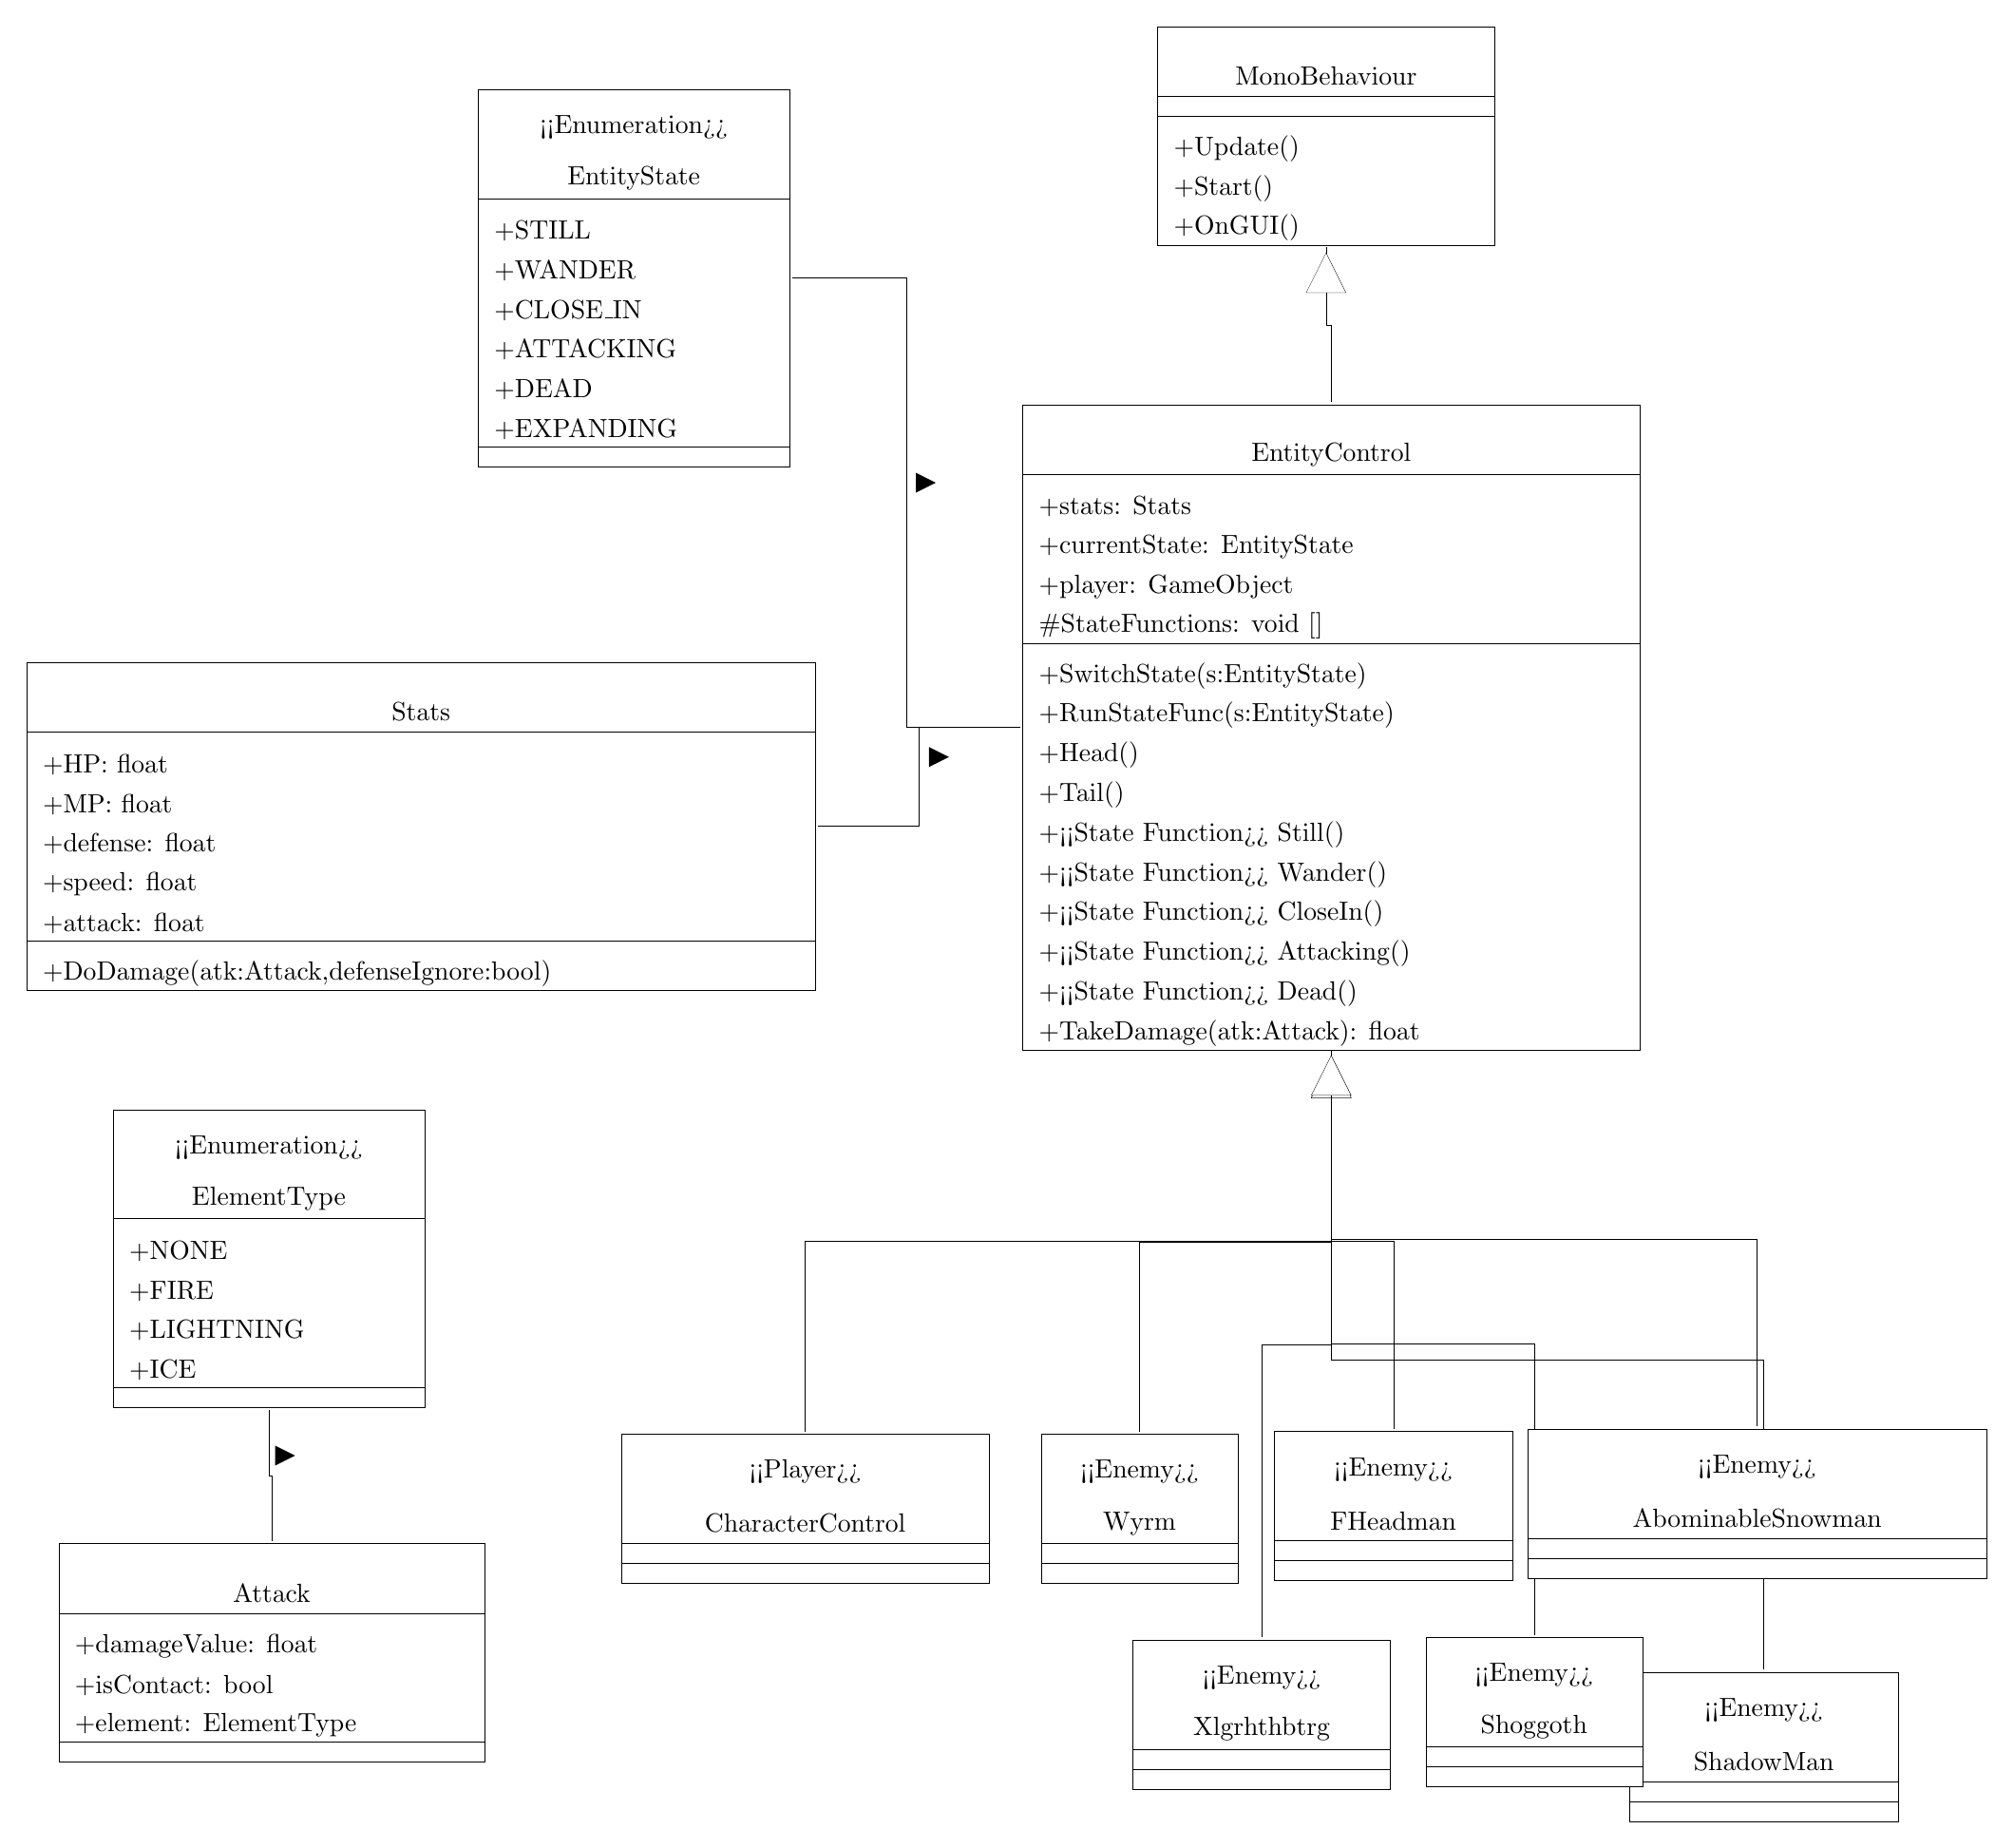
\begin{tikzpicture}
\pgftransformxscale{0.663512}
\pgftransformyscale{-0.663512}
\definecolor{dialinecolor}{rgb}{0.000000, 0.000000, 0.000000}
\pgfsetstrokecolor{dialinecolor}
\definecolor{dialinecolor}{rgb}{1.000000, 1.000000, 1.000000}
\pgfsetfillcolor{dialinecolor}
\pgfsetlinewidth{0.100000\du}
\pgfsetdash{}{0pt}
\definecolor{dialinecolor}{rgb}{1.000000, 1.000000, 1.000000}
\pgfsetfillcolor{dialinecolor}
\fill (-6.800000\du,4.250000\du)--(-6.800000\du,5.650000\du)--(5.635000\du,5.650000\du)--(5.635000\du,4.250000\du)--cycle;
\definecolor{dialinecolor}{rgb}{0.000000, 0.000000, 0.000000}
\pgfsetstrokecolor{dialinecolor}
\draw (-6.800000\du,4.250000\du)--(-6.800000\du,5.650000\du)--(5.635000\du,5.650000\du)--(5.635000\du,4.250000\du)--cycle;
% setfont left to latex
\definecolor{dialinecolor}{rgb}{0.000000, 0.000000, 0.000000}
\pgfsetstrokecolor{dialinecolor}
\node at (-0.582500\du,5.250000\du){EntityControl};
\definecolor{dialinecolor}{rgb}{1.000000, 1.000000, 1.000000}
\pgfsetfillcolor{dialinecolor}
\fill (-6.800000\du,5.650000\du)--(-6.800000\du,9.050000\du)--(5.635000\du,9.050000\du)--(5.635000\du,5.650000\du)--cycle;
\definecolor{dialinecolor}{rgb}{0.000000, 0.000000, 0.000000}
\pgfsetstrokecolor{dialinecolor}
\draw (-6.800000\du,5.650000\du)--(-6.800000\du,9.050000\du)--(5.635000\du,9.050000\du)--(5.635000\du,5.650000\du)--cycle;
% setfont left to latex
\definecolor{dialinecolor}{rgb}{0.000000, 0.000000, 0.000000}
\pgfsetstrokecolor{dialinecolor}
\node[anchor=west] at (-6.650000\du,6.310000\du){+stats: Stats};
% setfont left to latex
\definecolor{dialinecolor}{rgb}{0.000000, 0.000000, 0.000000}
\pgfsetstrokecolor{dialinecolor}
\node[anchor=west] at (-6.650000\du,7.110000\du){+currentState: EntityState};
% setfont left to latex
\definecolor{dialinecolor}{rgb}{0.000000, 0.000000, 0.000000}
\pgfsetstrokecolor{dialinecolor}
\node[anchor=west] at (-6.650000\du,7.910000\du){+player: GameObject};
% setfont left to latex
\definecolor{dialinecolor}{rgb}{0.000000, 0.000000, 0.000000}
\pgfsetstrokecolor{dialinecolor}
\node[anchor=west] at (-6.650000\du,8.710000\du){\#StateFunctions: void \ensuremath{[}\ensuremath{]}};
\definecolor{dialinecolor}{rgb}{1.000000, 1.000000, 1.000000}
\pgfsetfillcolor{dialinecolor}
\fill (-6.800000\du,9.050000\du)--(-6.800000\du,17.250000\du)--(5.635000\du,17.250000\du)--(5.635000\du,9.050000\du)--cycle;
\definecolor{dialinecolor}{rgb}{0.000000, 0.000000, 0.000000}
\pgfsetstrokecolor{dialinecolor}
\draw (-6.800000\du,9.050000\du)--(-6.800000\du,17.250000\du)--(5.635000\du,17.250000\du)--(5.635000\du,9.050000\du)--cycle;
% setfont left to latex
\definecolor{dialinecolor}{rgb}{0.000000, 0.000000, 0.000000}
\pgfsetstrokecolor{dialinecolor}
\node[anchor=west] at (-6.650000\du,9.710000\du){+SwitchState(s:EntityState)};
% setfont left to latex
\definecolor{dialinecolor}{rgb}{0.000000, 0.000000, 0.000000}
\pgfsetstrokecolor{dialinecolor}
\node[anchor=west] at (-6.650000\du,10.510000\du){+RunStateFunc(s:EntityState)};
% setfont left to latex
\definecolor{dialinecolor}{rgb}{0.000000, 0.000000, 0.000000}
\pgfsetstrokecolor{dialinecolor}
\node[anchor=west] at (-6.650000\du,11.310000\du){+Head()};
% setfont left to latex
\definecolor{dialinecolor}{rgb}{0.000000, 0.000000, 0.000000}
\pgfsetstrokecolor{dialinecolor}
\node[anchor=west] at (-6.650000\du,12.110000\du){+Tail()};
% setfont left to latex
\definecolor{dialinecolor}{rgb}{0.000000, 0.000000, 0.000000}
\pgfsetstrokecolor{dialinecolor}
\node[anchor=west] at (-6.650000\du,12.910000\du){+<<State Function>> Still()};
% setfont left to latex
\definecolor{dialinecolor}{rgb}{0.000000, 0.000000, 0.000000}
\pgfsetstrokecolor{dialinecolor}
\node[anchor=west] at (-6.650000\du,13.710000\du){+<<State Function>> Wander()};
% setfont left to latex
\definecolor{dialinecolor}{rgb}{0.000000, 0.000000, 0.000000}
\pgfsetstrokecolor{dialinecolor}
\node[anchor=west] at (-6.650000\du,14.510000\du){+<<State Function>> CloseIn()};
% setfont left to latex
\definecolor{dialinecolor}{rgb}{0.000000, 0.000000, 0.000000}
\pgfsetstrokecolor{dialinecolor}
\node[anchor=west] at (-6.650000\du,15.310000\du){+<<State Function>> Attacking()};
% setfont left to latex
\definecolor{dialinecolor}{rgb}{0.000000, 0.000000, 0.000000}
\pgfsetstrokecolor{dialinecolor}
\node[anchor=west] at (-6.650000\du,16.110000\du){+<<State Function>> Dead()};
% setfont left to latex
\definecolor{dialinecolor}{rgb}{0.000000, 0.000000, 0.000000}
\pgfsetstrokecolor{dialinecolor}
\node[anchor=west] at (-6.650000\du,16.910000\du){+TakeDamage(atk:Attack): float};
\pgfsetlinewidth{0.100000\du}
\pgfsetdash{}{0pt}
\definecolor{dialinecolor}{rgb}{1.000000, 1.000000, 1.000000}
\pgfsetfillcolor{dialinecolor}
\fill (-4.084280\du,-3.371880\du)--(-4.084280\du,-1.971880\du)--(2.710720\du,-1.971880\du)--(2.710720\du,-3.371880\du)--cycle;
\definecolor{dialinecolor}{rgb}{0.000000, 0.000000, 0.000000}
\pgfsetstrokecolor{dialinecolor}
\draw (-4.084280\du,-3.371880\du)--(-4.084280\du,-1.971880\du)--(2.710720\du,-1.971880\du)--(2.710720\du,-3.371880\du)--cycle;
% setfont left to latex
\definecolor{dialinecolor}{rgb}{0.000000, 0.000000, 0.000000}
\pgfsetstrokecolor{dialinecolor}
\node at (-0.686780\du,-2.371880\du){MonoBehaviour};
\definecolor{dialinecolor}{rgb}{1.000000, 1.000000, 1.000000}
\pgfsetfillcolor{dialinecolor}
\fill (-4.084280\du,-1.971880\du)--(-4.084280\du,-1.571880\du)--(2.710720\du,-1.571880\du)--(2.710720\du,-1.971880\du)--cycle;
\definecolor{dialinecolor}{rgb}{0.000000, 0.000000, 0.000000}
\pgfsetstrokecolor{dialinecolor}
\draw (-4.084280\du,-1.971880\du)--(-4.084280\du,-1.571880\du)--(2.710720\du,-1.571880\du)--(2.710720\du,-1.971880\du)--cycle;
\definecolor{dialinecolor}{rgb}{1.000000, 1.000000, 1.000000}
\pgfsetfillcolor{dialinecolor}
\fill (-4.084280\du,-1.571880\du)--(-4.084280\du,1.028120\du)--(2.710720\du,1.028120\du)--(2.710720\du,-1.571880\du)--cycle;
\definecolor{dialinecolor}{rgb}{0.000000, 0.000000, 0.000000}
\pgfsetstrokecolor{dialinecolor}
\draw (-4.084280\du,-1.571880\du)--(-4.084280\du,1.028120\du)--(2.710720\du,1.028120\du)--(2.710720\du,-1.571880\du)--cycle;
% setfont left to latex
\definecolor{dialinecolor}{rgb}{0.000000, 0.000000, 0.000000}
\pgfsetstrokecolor{dialinecolor}
\node[anchor=west] at (-3.934280\du,-0.911880\du){+Update()};
% setfont left to latex
\definecolor{dialinecolor}{rgb}{0.000000, 0.000000, 0.000000}
\pgfsetstrokecolor{dialinecolor}
\node[anchor=west] at (-3.934280\du,-0.111880\du){+Start()};
% setfont left to latex
\definecolor{dialinecolor}{rgb}{0.000000, 0.000000, 0.000000}
\pgfsetstrokecolor{dialinecolor}
\node[anchor=west] at (-3.934280\du,0.688120\du){+OnGUI()};
\pgfsetlinewidth{0.100000\du}
\pgfsetdash{}{0pt}
\pgfsetmiterjoin
\pgfsetbuttcap
{
\definecolor{dialinecolor}{rgb}{0.000000, 0.000000, 0.000000}
\pgfsetfillcolor{dialinecolor}
% was here!!!
\definecolor{dialinecolor}{rgb}{0.000000, 0.000000, 0.000000}
\pgfsetstrokecolor{dialinecolor}
\draw (-0.686780\du,1.078395\du)--(-0.686780\du,2.638997\du)--(-0.582500\du,2.638997\du)--(-0.582500\du,4.199600\du);
}
\definecolor{dialinecolor}{rgb}{0.000000, 0.000000, 0.000000}
\pgfsetstrokecolor{dialinecolor}
\draw (-0.686780\du,1.990198\du)--(-0.686780\du,2.638997\du)--(-0.582500\du,2.638997\du)--(-0.582500\du,4.199600\du);
\pgfsetmiterjoin
\definecolor{dialinecolor}{rgb}{1.000000, 1.000000, 1.000000}
\pgfsetfillcolor{dialinecolor}
\fill (-0.286780\du,1.990198\du)--(-0.686780\du,1.190198\du)--(-1.086780\du,1.990198\du)--cycle;
\pgfsetlinewidth{0.100000\du}
\pgfsetdash{}{0pt}
\pgfsetmiterjoin
\definecolor{dialinecolor}{rgb}{0.000000, 0.000000, 0.000000}
\pgfsetstrokecolor{dialinecolor}
\draw (-0.286780\du,1.990198\du)--(-0.686780\du,1.190198\du)--(-1.086780\du,1.990198\du)--cycle;
% setfont left to latex
\pgfsetlinewidth{0.100000\du}
\pgfsetdash{}{0pt}
\definecolor{dialinecolor}{rgb}{1.000000, 1.000000, 1.000000}
\pgfsetfillcolor{dialinecolor}
\fill (-17.771800\du,-2.109380\du)--(-17.771800\du,0.090620\du)--(-11.496800\du,0.090620\du)--(-11.496800\du,-2.109380\du)--cycle;
\definecolor{dialinecolor}{rgb}{0.000000, 0.000000, 0.000000}
\pgfsetstrokecolor{dialinecolor}
\draw (-17.771800\du,-2.109380\du)--(-17.771800\du,0.090620\du)--(-11.496800\du,0.090620\du)--(-11.496800\du,-2.109380\du)--cycle;
% setfont left to latex
\definecolor{dialinecolor}{rgb}{0.000000, 0.000000, 0.000000}
\pgfsetstrokecolor{dialinecolor}
\node at (-14.634300\du,-1.349380\du){<<Enumeration>>};
% setfont left to latex
\definecolor{dialinecolor}{rgb}{0.000000, 0.000000, 0.000000}
\pgfsetstrokecolor{dialinecolor}
\node at (-14.634300\du,-0.309380\du){EntityState};
\definecolor{dialinecolor}{rgb}{1.000000, 1.000000, 1.000000}
\pgfsetfillcolor{dialinecolor}
\fill (-17.771800\du,0.090620\du)--(-17.771800\du,5.090620\du)--(-11.496800\du,5.090620\du)--(-11.496800\du,0.090620\du)--cycle;
\definecolor{dialinecolor}{rgb}{0.000000, 0.000000, 0.000000}
\pgfsetstrokecolor{dialinecolor}
\draw (-17.771800\du,0.090620\du)--(-17.771800\du,5.090620\du)--(-11.496800\du,5.090620\du)--(-11.496800\du,0.090620\du)--cycle;
% setfont left to latex
\definecolor{dialinecolor}{rgb}{0.000000, 0.000000, 0.000000}
\pgfsetstrokecolor{dialinecolor}
\node[anchor=west] at (-17.621800\du,0.750620\du){+STILL};
% setfont left to latex
\definecolor{dialinecolor}{rgb}{0.000000, 0.000000, 0.000000}
\pgfsetstrokecolor{dialinecolor}
\node[anchor=west] at (-17.621800\du,1.550620\du){+WANDER};
% setfont left to latex
\definecolor{dialinecolor}{rgb}{0.000000, 0.000000, 0.000000}
\pgfsetstrokecolor{dialinecolor}
\node[anchor=west] at (-17.621800\du,2.350620\du){+CLOSE\_IN};
% setfont left to latex
\definecolor{dialinecolor}{rgb}{0.000000, 0.000000, 0.000000}
\pgfsetstrokecolor{dialinecolor}
\node[anchor=west] at (-17.621800\du,3.150620\du){+ATTACKING};
% setfont left to latex
\definecolor{dialinecolor}{rgb}{0.000000, 0.000000, 0.000000}
\pgfsetstrokecolor{dialinecolor}
\node[anchor=west] at (-17.621800\du,3.950620\du){+DEAD};
% setfont left to latex
\definecolor{dialinecolor}{rgb}{0.000000, 0.000000, 0.000000}
\pgfsetstrokecolor{dialinecolor}
\node[anchor=west] at (-17.621800\du,4.750620\du){+EXPANDING};
\definecolor{dialinecolor}{rgb}{1.000000, 1.000000, 1.000000}
\pgfsetfillcolor{dialinecolor}
\fill (-17.771800\du,5.090620\du)--(-17.771800\du,5.490620\du)--(-11.496800\du,5.490620\du)--(-11.496800\du,5.090620\du)--cycle;
\definecolor{dialinecolor}{rgb}{0.000000, 0.000000, 0.000000}
\pgfsetstrokecolor{dialinecolor}
\draw (-17.771800\du,5.090620\du)--(-17.771800\du,5.490620\du)--(-11.496800\du,5.490620\du)--(-11.496800\du,5.090620\du)--cycle;
\pgfsetlinewidth{0.100000\du}
\pgfsetdash{}{0pt}
\pgfsetmiterjoin
\pgfsetbuttcap
{
\definecolor{dialinecolor}{rgb}{0.000000, 0.000000, 0.000000}
\pgfsetfillcolor{dialinecolor}
% was here!!!
\definecolor{dialinecolor}{rgb}{0.000000, 0.000000, 0.000000}
\pgfsetstrokecolor{dialinecolor}
\draw (-11.446411\du,1.690620\du)--(-9.148397\du,1.690620\du)--(-9.148397\du,10.750000\du)--(-6.850383\du,10.750000\du);
}
% setfont left to latex
\definecolor{dialinecolor}{rgb}{0.000000, 0.000000, 0.000000}
\pgfsetstrokecolor{dialinecolor}
\node[anchor=west] at (-9.048397\du,6.020310\du){};
\definecolor{dialinecolor}{rgb}{0.000000, 0.000000, 0.000000}
\pgfsetfillcolor{dialinecolor}
\fill (-8.948397\du,6.020310\du)--(-8.948397\du,5.620310\du)--(-8.548397\du,5.820310\du)--cycle;
\definecolor{dialinecolor}{rgb}{0.000000, 0.000000, 0.000000}
\pgfsetstrokecolor{dialinecolor}
\node[anchor=west] at (-11.246411\du,1.490620\du){};
\definecolor{dialinecolor}{rgb}{0.000000, 0.000000, 0.000000}
\pgfsetstrokecolor{dialinecolor}
\node[anchor=east] at (-7.050383\du,10.550000\du){};
\pgfsetlinewidth{0.100000\du}
\pgfsetdash{}{0pt}
\definecolor{dialinecolor}{rgb}{1.000000, 1.000000, 1.000000}
\pgfsetfillcolor{dialinecolor}
\fill (-26.871800\du,9.440620\du)--(-26.871800\du,10.840620\du)--(-10.971800\du,10.840620\du)--(-10.971800\du,9.440620\du)--cycle;
\definecolor{dialinecolor}{rgb}{0.000000, 0.000000, 0.000000}
\pgfsetstrokecolor{dialinecolor}
\draw (-26.871800\du,9.440620\du)--(-26.871800\du,10.840620\du)--(-10.971800\du,10.840620\du)--(-10.971800\du,9.440620\du)--cycle;
% setfont left to latex
\definecolor{dialinecolor}{rgb}{0.000000, 0.000000, 0.000000}
\pgfsetstrokecolor{dialinecolor}
\node at (-18.921800\du,10.440620\du){Stats};
\definecolor{dialinecolor}{rgb}{1.000000, 1.000000, 1.000000}
\pgfsetfillcolor{dialinecolor}
\fill (-26.871800\du,10.840620\du)--(-26.871800\du,15.040620\du)--(-10.971800\du,15.040620\du)--(-10.971800\du,10.840620\du)--cycle;
\definecolor{dialinecolor}{rgb}{0.000000, 0.000000, 0.000000}
\pgfsetstrokecolor{dialinecolor}
\draw (-26.871800\du,10.840620\du)--(-26.871800\du,15.040620\du)--(-10.971800\du,15.040620\du)--(-10.971800\du,10.840620\du)--cycle;
% setfont left to latex
\definecolor{dialinecolor}{rgb}{0.000000, 0.000000, 0.000000}
\pgfsetstrokecolor{dialinecolor}
\node[anchor=west] at (-26.721800\du,11.500620\du){+HP: float};
% setfont left to latex
\definecolor{dialinecolor}{rgb}{0.000000, 0.000000, 0.000000}
\pgfsetstrokecolor{dialinecolor}
\node[anchor=west] at (-26.721800\du,12.300620\du){+MP: float};
% setfont left to latex
\definecolor{dialinecolor}{rgb}{0.000000, 0.000000, 0.000000}
\pgfsetstrokecolor{dialinecolor}
\node[anchor=west] at (-26.721800\du,13.100620\du){+defense: float};
% setfont left to latex
\definecolor{dialinecolor}{rgb}{0.000000, 0.000000, 0.000000}
\pgfsetstrokecolor{dialinecolor}
\node[anchor=west] at (-26.721800\du,13.900620\du){+speed: float};
% setfont left to latex
\definecolor{dialinecolor}{rgb}{0.000000, 0.000000, 0.000000}
\pgfsetstrokecolor{dialinecolor}
\node[anchor=west] at (-26.721800\du,14.700620\du){+attack: float};
\definecolor{dialinecolor}{rgb}{1.000000, 1.000000, 1.000000}
\pgfsetfillcolor{dialinecolor}
\fill (-26.871800\du,15.040620\du)--(-26.871800\du,16.040620\du)--(-10.971800\du,16.040620\du)--(-10.971800\du,15.040620\du)--cycle;
\definecolor{dialinecolor}{rgb}{0.000000, 0.000000, 0.000000}
\pgfsetstrokecolor{dialinecolor}
\draw (-26.871800\du,15.040620\du)--(-26.871800\du,16.040620\du)--(-10.971800\du,16.040620\du)--(-10.971800\du,15.040620\du)--cycle;
% setfont left to latex
\definecolor{dialinecolor}{rgb}{0.000000, 0.000000, 0.000000}
\pgfsetstrokecolor{dialinecolor}
\node[anchor=west] at (-26.721800\du,15.700620\du){+DoDamage(atk:Attack,defenseIgnore:bool)};
\pgfsetlinewidth{0.100000\du}
\pgfsetdash{}{0pt}
\definecolor{dialinecolor}{rgb}{1.000000, 1.000000, 1.000000}
\pgfsetfillcolor{dialinecolor}
\fill (-26.221800\du,27.190600\du)--(-26.221800\du,28.590600\du)--(-17.636800\du,28.590600\du)--(-17.636800\du,27.190600\du)--cycle;
\definecolor{dialinecolor}{rgb}{0.000000, 0.000000, 0.000000}
\pgfsetstrokecolor{dialinecolor}
\draw (-26.221800\du,27.190600\du)--(-26.221800\du,28.590600\du)--(-17.636800\du,28.590600\du)--(-17.636800\du,27.190600\du)--cycle;
% setfont left to latex
\definecolor{dialinecolor}{rgb}{0.000000, 0.000000, 0.000000}
\pgfsetstrokecolor{dialinecolor}
\node at (-21.929300\du,28.190600\du){Attack};
\definecolor{dialinecolor}{rgb}{1.000000, 1.000000, 1.000000}
\pgfsetfillcolor{dialinecolor}
\fill (-26.221800\du,28.590600\du)--(-26.221800\du,31.190600\du)--(-17.636800\du,31.190600\du)--(-17.636800\du,28.590600\du)--cycle;
\definecolor{dialinecolor}{rgb}{0.000000, 0.000000, 0.000000}
\pgfsetstrokecolor{dialinecolor}
\draw (-26.221800\du,28.590600\du)--(-26.221800\du,31.190600\du)--(-17.636800\du,31.190600\du)--(-17.636800\du,28.590600\du)--cycle;
% setfont left to latex
\definecolor{dialinecolor}{rgb}{0.000000, 0.000000, 0.000000}
\pgfsetstrokecolor{dialinecolor}
\node[anchor=west] at (-26.071800\du,29.250600\du){+damageValue: float};
% setfont left to latex
\definecolor{dialinecolor}{rgb}{0.000000, 0.000000, 0.000000}
\pgfsetstrokecolor{dialinecolor}
\node[anchor=west] at (-26.071800\du,30.050600\du){+isContact: bool};
% setfont left to latex
\definecolor{dialinecolor}{rgb}{0.000000, 0.000000, 0.000000}
\pgfsetstrokecolor{dialinecolor}
\node[anchor=west] at (-26.071800\du,30.850600\du){+element: ElementType};
\definecolor{dialinecolor}{rgb}{1.000000, 1.000000, 1.000000}
\pgfsetfillcolor{dialinecolor}
\fill (-26.221800\du,31.190600\du)--(-26.221800\du,31.590600\du)--(-17.636800\du,31.590600\du)--(-17.636800\du,31.190600\du)--cycle;
\definecolor{dialinecolor}{rgb}{0.000000, 0.000000, 0.000000}
\pgfsetstrokecolor{dialinecolor}
\draw (-26.221800\du,31.190600\du)--(-26.221800\du,31.590600\du)--(-17.636800\du,31.590600\du)--(-17.636800\du,31.190600\du)--cycle;
\pgfsetlinewidth{0.100000\du}
\pgfsetdash{}{0pt}
\definecolor{dialinecolor}{rgb}{1.000000, 1.000000, 1.000000}
\pgfsetfillcolor{dialinecolor}
\fill (-25.126800\du,18.445600\du)--(-25.126800\du,20.645600\du)--(-18.851800\du,20.645600\du)--(-18.851800\du,18.445600\du)--cycle;
\definecolor{dialinecolor}{rgb}{0.000000, 0.000000, 0.000000}
\pgfsetstrokecolor{dialinecolor}
\draw (-25.126800\du,18.445600\du)--(-25.126800\du,20.645600\du)--(-18.851800\du,20.645600\du)--(-18.851800\du,18.445600\du)--cycle;
% setfont left to latex
\definecolor{dialinecolor}{rgb}{0.000000, 0.000000, 0.000000}
\pgfsetstrokecolor{dialinecolor}
\node at (-21.989300\du,19.205600\du){<<Enumeration>>};
% setfont left to latex
\definecolor{dialinecolor}{rgb}{0.000000, 0.000000, 0.000000}
\pgfsetstrokecolor{dialinecolor}
\node at (-21.989300\du,20.245600\du){ElementType};
\definecolor{dialinecolor}{rgb}{1.000000, 1.000000, 1.000000}
\pgfsetfillcolor{dialinecolor}
\fill (-25.126800\du,20.645600\du)--(-25.126800\du,24.045600\du)--(-18.851800\du,24.045600\du)--(-18.851800\du,20.645600\du)--cycle;
\definecolor{dialinecolor}{rgb}{0.000000, 0.000000, 0.000000}
\pgfsetstrokecolor{dialinecolor}
\draw (-25.126800\du,20.645600\du)--(-25.126800\du,24.045600\du)--(-18.851800\du,24.045600\du)--(-18.851800\du,20.645600\du)--cycle;
% setfont left to latex
\definecolor{dialinecolor}{rgb}{0.000000, 0.000000, 0.000000}
\pgfsetstrokecolor{dialinecolor}
\node[anchor=west] at (-24.976800\du,21.305600\du){+NONE};
% setfont left to latex
\definecolor{dialinecolor}{rgb}{0.000000, 0.000000, 0.000000}
\pgfsetstrokecolor{dialinecolor}
\node[anchor=west] at (-24.976800\du,22.105600\du){+FIRE};
% setfont left to latex
\definecolor{dialinecolor}{rgb}{0.000000, 0.000000, 0.000000}
\pgfsetstrokecolor{dialinecolor}
\node[anchor=west] at (-24.976800\du,22.905600\du){+LIGHTNING};
% setfont left to latex
\definecolor{dialinecolor}{rgb}{0.000000, 0.000000, 0.000000}
\pgfsetstrokecolor{dialinecolor}
\node[anchor=west] at (-24.976800\du,23.705600\du){+ICE};
\definecolor{dialinecolor}{rgb}{1.000000, 1.000000, 1.000000}
\pgfsetfillcolor{dialinecolor}
\fill (-25.126800\du,24.045600\du)--(-25.126800\du,24.445600\du)--(-18.851800\du,24.445600\du)--(-18.851800\du,24.045600\du)--cycle;
\definecolor{dialinecolor}{rgb}{0.000000, 0.000000, 0.000000}
\pgfsetstrokecolor{dialinecolor}
\draw (-25.126800\du,24.045600\du)--(-25.126800\du,24.445600\du)--(-18.851800\du,24.445600\du)--(-18.851800\du,24.045600\du)--cycle;
\pgfsetlinewidth{0.100000\du}
\pgfsetdash{}{0pt}
\pgfsetmiterjoin
\pgfsetbuttcap
{
\definecolor{dialinecolor}{rgb}{0.000000, 0.000000, 0.000000}
\pgfsetfillcolor{dialinecolor}
% was here!!!
\definecolor{dialinecolor}{rgb}{0.000000, 0.000000, 0.000000}
\pgfsetstrokecolor{dialinecolor}
\draw (-21.929300\du,27.140325\du)--(-21.929300\du,25.818149\du)--(-21.989300\du,25.818149\du)--(-21.989300\du,24.495972\du);
}
% setfont left to latex
\definecolor{dialinecolor}{rgb}{0.000000, 0.000000, 0.000000}
\pgfsetstrokecolor{dialinecolor}
\node at (-21.959300\du,25.618149\du){};
\definecolor{dialinecolor}{rgb}{0.000000, 0.000000, 0.000000}
\pgfsetfillcolor{dialinecolor}
\fill (-21.859300\du,25.618149\du)--(-21.859300\du,25.218149\du)--(-21.459300\du,25.418149\du)--cycle;
\definecolor{dialinecolor}{rgb}{0.000000, 0.000000, 0.000000}
\pgfsetstrokecolor{dialinecolor}
\node[anchor=west] at (-21.729300\du,26.940325\du){};
\definecolor{dialinecolor}{rgb}{0.000000, 0.000000, 0.000000}
\pgfsetstrokecolor{dialinecolor}
\node[anchor=west] at (-21.789300\du,25.095972\du){};
\pgfsetlinewidth{0.100000\du}
\pgfsetdash{}{0pt}
\pgfsetmiterjoin
\pgfsetbuttcap
{
\definecolor{dialinecolor}{rgb}{0.000000, 0.000000, 0.000000}
\pgfsetfillcolor{dialinecolor}
% was here!!!
\definecolor{dialinecolor}{rgb}{0.000000, 0.000000, 0.000000}
\pgfsetstrokecolor{dialinecolor}
\draw (-6.850383\du,10.750000\du)--(-8.885847\du,10.750000\du)--(-8.885847\du,12.740620\du)--(-10.921312\du,12.740620\du);
}
% setfont left to latex
\definecolor{dialinecolor}{rgb}{0.000000, 0.000000, 0.000000}
\pgfsetstrokecolor{dialinecolor}
\node[anchor=west] at (-8.785847\du,11.545310\du){};
\definecolor{dialinecolor}{rgb}{0.000000, 0.000000, 0.000000}
\pgfsetfillcolor{dialinecolor}
\fill (-8.685847\du,11.545310\du)--(-8.685847\du,11.145310\du)--(-8.285847\du,11.345310\du)--cycle;
\definecolor{dialinecolor}{rgb}{0.000000, 0.000000, 0.000000}
\pgfsetstrokecolor{dialinecolor}
\node[anchor=east] at (-7.050383\du,10.550000\du){};
\definecolor{dialinecolor}{rgb}{0.000000, 0.000000, 0.000000}
\pgfsetstrokecolor{dialinecolor}
\node[anchor=west] at (-10.721312\du,12.540620\du){};
\pgfsetlinewidth{0.100000\du}
\pgfsetdash{}{0pt}
\definecolor{dialinecolor}{rgb}{1.000000, 1.000000, 1.000000}
\pgfsetfillcolor{dialinecolor}
\fill (-1.726770\du,24.933100\du)--(-1.726770\du,27.133100\du)--(3.063230\du,27.133100\du)--(3.063230\du,24.933100\du)--cycle;
\definecolor{dialinecolor}{rgb}{0.000000, 0.000000, 0.000000}
\pgfsetstrokecolor{dialinecolor}
\draw (-1.726770\du,24.933100\du)--(-1.726770\du,27.133100\du)--(3.063230\du,27.133100\du)--(3.063230\du,24.933100\du)--cycle;
% setfont left to latex
\definecolor{dialinecolor}{rgb}{0.000000, 0.000000, 0.000000}
\pgfsetstrokecolor{dialinecolor}
\node at (0.668230\du,25.693100\du){<<Enemy>>};
% setfont left to latex
\definecolor{dialinecolor}{rgb}{0.000000, 0.000000, 0.000000}
\pgfsetstrokecolor{dialinecolor}
\node at (0.668230\du,26.733100\du){FHeadman};
\definecolor{dialinecolor}{rgb}{1.000000, 1.000000, 1.000000}
\pgfsetfillcolor{dialinecolor}
\fill (-1.726770\du,27.133100\du)--(-1.726770\du,27.533100\du)--(3.063230\du,27.533100\du)--(3.063230\du,27.133100\du)--cycle;
\definecolor{dialinecolor}{rgb}{0.000000, 0.000000, 0.000000}
\pgfsetstrokecolor{dialinecolor}
\draw (-1.726770\du,27.133100\du)--(-1.726770\du,27.533100\du)--(3.063230\du,27.533100\du)--(3.063230\du,27.133100\du)--cycle;
\definecolor{dialinecolor}{rgb}{1.000000, 1.000000, 1.000000}
\pgfsetfillcolor{dialinecolor}
\fill (-1.726770\du,27.533100\du)--(-1.726770\du,27.933100\du)--(3.063230\du,27.933100\du)--(3.063230\du,27.533100\du)--cycle;
\definecolor{dialinecolor}{rgb}{0.000000, 0.000000, 0.000000}
\pgfsetstrokecolor{dialinecolor}
\draw (-1.726770\du,27.533100\du)--(-1.726770\du,27.933100\du)--(3.063230\du,27.933100\du)--(3.063230\du,27.533100\du)--cycle;
\pgfsetlinewidth{0.100000\du}
\pgfsetdash{}{0pt}
\pgfsetmiterjoin
\pgfsetbuttcap
{
\definecolor{dialinecolor}{rgb}{0.000000, 0.000000, 0.000000}
\pgfsetfillcolor{dialinecolor}
% was here!!!
\definecolor{dialinecolor}{rgb}{0.000000, 0.000000, 0.000000}
\pgfsetstrokecolor{dialinecolor}
\draw (-0.582500\du,17.300400\du)--(-0.582500\du,21.091561\du)--(0.668230\du,21.091561\du)--(0.668230\du,24.882722\du);
}
\definecolor{dialinecolor}{rgb}{0.000000, 0.000000, 0.000000}
\pgfsetstrokecolor{dialinecolor}
\draw (-0.582500\du,18.212203\du)--(-0.582500\du,21.091561\du)--(0.668230\du,21.091561\du)--(0.668230\du,24.882722\du);
\pgfsetmiterjoin
\definecolor{dialinecolor}{rgb}{1.000000, 1.000000, 1.000000}
\pgfsetfillcolor{dialinecolor}
\fill (-0.182500\du,18.212203\du)--(-0.582500\du,17.412203\du)--(-0.982500\du,18.212203\du)--cycle;
\pgfsetlinewidth{0.100000\du}
\pgfsetdash{}{0pt}
\pgfsetmiterjoin
\definecolor{dialinecolor}{rgb}{0.000000, 0.000000, 0.000000}
\pgfsetstrokecolor{dialinecolor}
\draw (-0.182500\du,18.212203\du)--(-0.582500\du,17.412203\du)--(-0.982500\du,18.212203\du)--cycle;
% setfont left to latex
\pgfsetlinewidth{0.100000\du}
\pgfsetdash{}{0pt}
\definecolor{dialinecolor}{rgb}{1.000000, 1.000000, 1.000000}
\pgfsetfillcolor{dialinecolor}
\fill (5.423220\du,29.783100\du)--(5.423220\du,31.983100\du)--(10.840720\du,31.983100\du)--(10.840720\du,29.783100\du)--cycle;
\definecolor{dialinecolor}{rgb}{0.000000, 0.000000, 0.000000}
\pgfsetstrokecolor{dialinecolor}
\draw (5.423220\du,29.783100\du)--(5.423220\du,31.983100\du)--(10.840720\du,31.983100\du)--(10.840720\du,29.783100\du)--cycle;
% setfont left to latex
\definecolor{dialinecolor}{rgb}{0.000000, 0.000000, 0.000000}
\pgfsetstrokecolor{dialinecolor}
\node at (8.131970\du,30.543100\du){<<Enemy>>};
% setfont left to latex
\definecolor{dialinecolor}{rgb}{0.000000, 0.000000, 0.000000}
\pgfsetstrokecolor{dialinecolor}
\node at (8.131970\du,31.583100\du){ShadowMan};
\definecolor{dialinecolor}{rgb}{1.000000, 1.000000, 1.000000}
\pgfsetfillcolor{dialinecolor}
\fill (5.423220\du,31.983100\du)--(5.423220\du,32.383100\du)--(10.840720\du,32.383100\du)--(10.840720\du,31.983100\du)--cycle;
\definecolor{dialinecolor}{rgb}{0.000000, 0.000000, 0.000000}
\pgfsetstrokecolor{dialinecolor}
\draw (5.423220\du,31.983100\du)--(5.423220\du,32.383100\du)--(10.840720\du,32.383100\du)--(10.840720\du,31.983100\du)--cycle;
\definecolor{dialinecolor}{rgb}{1.000000, 1.000000, 1.000000}
\pgfsetfillcolor{dialinecolor}
\fill (5.423220\du,32.383100\du)--(5.423220\du,32.783100\du)--(10.840720\du,32.783100\du)--(10.840720\du,32.383100\du)--cycle;
\definecolor{dialinecolor}{rgb}{0.000000, 0.000000, 0.000000}
\pgfsetstrokecolor{dialinecolor}
\draw (5.423220\du,32.383100\du)--(5.423220\du,32.783100\du)--(10.840720\du,32.783100\du)--(10.840720\du,32.383100\du)--cycle;
\pgfsetlinewidth{0.100000\du}
\pgfsetdash{}{0pt}
\definecolor{dialinecolor}{rgb}{1.000000, 1.000000, 1.000000}
\pgfsetfillcolor{dialinecolor}
\fill (1.323220\du,29.083100\du)--(1.323220\du,31.283100\du)--(5.683220\du,31.283100\du)--(5.683220\du,29.083100\du)--cycle;
\definecolor{dialinecolor}{rgb}{0.000000, 0.000000, 0.000000}
\pgfsetstrokecolor{dialinecolor}
\draw (1.323220\du,29.083100\du)--(1.323220\du,31.283100\du)--(5.683220\du,31.283100\du)--(5.683220\du,29.083100\du)--cycle;
% setfont left to latex
\definecolor{dialinecolor}{rgb}{0.000000, 0.000000, 0.000000}
\pgfsetstrokecolor{dialinecolor}
\node at (3.503220\du,29.843100\du){<<Enemy>>};
% setfont left to latex
\definecolor{dialinecolor}{rgb}{0.000000, 0.000000, 0.000000}
\pgfsetstrokecolor{dialinecolor}
\node at (3.503220\du,30.883100\du){Shoggoth};
\definecolor{dialinecolor}{rgb}{1.000000, 1.000000, 1.000000}
\pgfsetfillcolor{dialinecolor}
\fill (1.323220\du,31.283100\du)--(1.323220\du,31.683100\du)--(5.683220\du,31.683100\du)--(5.683220\du,31.283100\du)--cycle;
\definecolor{dialinecolor}{rgb}{0.000000, 0.000000, 0.000000}
\pgfsetstrokecolor{dialinecolor}
\draw (1.323220\du,31.283100\du)--(1.323220\du,31.683100\du)--(5.683220\du,31.683100\du)--(5.683220\du,31.283100\du)--cycle;
\definecolor{dialinecolor}{rgb}{1.000000, 1.000000, 1.000000}
\pgfsetfillcolor{dialinecolor}
\fill (1.323220\du,31.683100\du)--(1.323220\du,32.083100\du)--(5.683220\du,32.083100\du)--(5.683220\du,31.683100\du)--cycle;
\definecolor{dialinecolor}{rgb}{0.000000, 0.000000, 0.000000}
\pgfsetstrokecolor{dialinecolor}
\draw (1.323220\du,31.683100\du)--(1.323220\du,32.083100\du)--(5.683220\du,32.083100\du)--(5.683220\du,31.683100\du)--cycle;
\pgfsetlinewidth{0.100000\du}
\pgfsetdash{}{0pt}
\definecolor{dialinecolor}{rgb}{1.000000, 1.000000, 1.000000}
\pgfsetfillcolor{dialinecolor}
\fill (-6.426770\du,24.983100\du)--(-6.426770\du,27.183100\du)--(-2.461770\du,27.183100\du)--(-2.461770\du,24.983100\du)--cycle;
\definecolor{dialinecolor}{rgb}{0.000000, 0.000000, 0.000000}
\pgfsetstrokecolor{dialinecolor}
\draw (-6.426770\du,24.983100\du)--(-6.426770\du,27.183100\du)--(-2.461770\du,27.183100\du)--(-2.461770\du,24.983100\du)--cycle;
% setfont left to latex
\definecolor{dialinecolor}{rgb}{0.000000, 0.000000, 0.000000}
\pgfsetstrokecolor{dialinecolor}
\node at (-4.444270\du,25.743100\du){<<Enemy>>};
% setfont left to latex
\definecolor{dialinecolor}{rgb}{0.000000, 0.000000, 0.000000}
\pgfsetstrokecolor{dialinecolor}
\node at (-4.444270\du,26.783100\du){Wyrm};
\definecolor{dialinecolor}{rgb}{1.000000, 1.000000, 1.000000}
\pgfsetfillcolor{dialinecolor}
\fill (-6.426770\du,27.183100\du)--(-6.426770\du,27.583100\du)--(-2.461770\du,27.583100\du)--(-2.461770\du,27.183100\du)--cycle;
\definecolor{dialinecolor}{rgb}{0.000000, 0.000000, 0.000000}
\pgfsetstrokecolor{dialinecolor}
\draw (-6.426770\du,27.183100\du)--(-6.426770\du,27.583100\du)--(-2.461770\du,27.583100\du)--(-2.461770\du,27.183100\du)--cycle;
\definecolor{dialinecolor}{rgb}{1.000000, 1.000000, 1.000000}
\pgfsetfillcolor{dialinecolor}
\fill (-6.426770\du,27.583100\du)--(-6.426770\du,27.983100\du)--(-2.461770\du,27.983100\du)--(-2.461770\du,27.583100\du)--cycle;
\definecolor{dialinecolor}{rgb}{0.000000, 0.000000, 0.000000}
\pgfsetstrokecolor{dialinecolor}
\draw (-6.426770\du,27.583100\du)--(-6.426770\du,27.983100\du)--(-2.461770\du,27.983100\du)--(-2.461770\du,27.583100\du)--cycle;
\pgfsetlinewidth{0.100000\du}
\pgfsetdash{}{0pt}
\pgfsetmiterjoin
\pgfsetbuttcap
{
\definecolor{dialinecolor}{rgb}{0.000000, 0.000000, 0.000000}
\pgfsetfillcolor{dialinecolor}
% was here!!!
\definecolor{dialinecolor}{rgb}{0.000000, 0.000000, 0.000000}
\pgfsetstrokecolor{dialinecolor}
\draw (-0.582500\du,17.300400\du)--(-0.582500\du,21.116561\du)--(-4.444270\du,21.116561\du)--(-4.444270\du,24.932722\du);
}
\definecolor{dialinecolor}{rgb}{0.000000, 0.000000, 0.000000}
\pgfsetstrokecolor{dialinecolor}
\draw (-0.582500\du,18.212203\du)--(-0.582500\du,21.116561\du)--(-4.444270\du,21.116561\du)--(-4.444270\du,24.932722\du);
\pgfsetmiterjoin
\definecolor{dialinecolor}{rgb}{1.000000, 1.000000, 1.000000}
\pgfsetfillcolor{dialinecolor}
\fill (-0.182500\du,18.212203\du)--(-0.582500\du,17.412203\du)--(-0.982500\du,18.212203\du)--cycle;
\pgfsetlinewidth{0.100000\du}
\pgfsetdash{}{0pt}
\pgfsetmiterjoin
\definecolor{dialinecolor}{rgb}{0.000000, 0.000000, 0.000000}
\pgfsetstrokecolor{dialinecolor}
\draw (-0.182500\du,18.212203\du)--(-0.582500\du,17.412203\du)--(-0.982500\du,18.212203\du)--cycle;
% setfont left to latex
\pgfsetlinewidth{0.100000\du}
\pgfsetdash{}{0pt}
\pgfsetmiterjoin
\pgfsetbuttcap
{
\definecolor{dialinecolor}{rgb}{0.000000, 0.000000, 0.000000}
\pgfsetfillcolor{dialinecolor}
% was here!!!
\definecolor{dialinecolor}{rgb}{0.000000, 0.000000, 0.000000}
\pgfsetstrokecolor{dialinecolor}
\draw (-0.582500\du,17.250000\du)--(-0.582500\du,23.491361\du)--(8.131970\du,23.491361\du)--(8.131970\du,29.732722\du);
}
\definecolor{dialinecolor}{rgb}{0.000000, 0.000000, 0.000000}
\pgfsetstrokecolor{dialinecolor}
\draw (-0.582500\du,18.161803\du)--(-0.582500\du,23.491361\du)--(8.131970\du,23.491361\du)--(8.131970\du,29.732722\du);
\pgfsetmiterjoin
\definecolor{dialinecolor}{rgb}{1.000000, 1.000000, 1.000000}
\pgfsetfillcolor{dialinecolor}
\fill (-0.182500\du,18.161803\du)--(-0.582500\du,17.361803\du)--(-0.982500\du,18.161803\du)--cycle;
\pgfsetlinewidth{0.100000\du}
\pgfsetdash{}{0pt}
\pgfsetmiterjoin
\definecolor{dialinecolor}{rgb}{0.000000, 0.000000, 0.000000}
\pgfsetstrokecolor{dialinecolor}
\draw (-0.182500\du,18.161803\du)--(-0.582500\du,17.361803\du)--(-0.982500\du,18.161803\du)--cycle;
% setfont left to latex
\pgfsetlinewidth{0.100000\du}
\pgfsetdash{}{0pt}
\pgfsetmiterjoin
\pgfsetbuttcap
{
\definecolor{dialinecolor}{rgb}{0.000000, 0.000000, 0.000000}
\pgfsetfillcolor{dialinecolor}
% was here!!!
\definecolor{dialinecolor}{rgb}{0.000000, 0.000000, 0.000000}
\pgfsetstrokecolor{dialinecolor}
\draw (-0.582500\du,17.300400\du)--(-0.582500\du,23.166561\du)--(3.503220\du,23.166561\du)--(3.503220\du,29.032722\du);
}
\definecolor{dialinecolor}{rgb}{0.000000, 0.000000, 0.000000}
\pgfsetstrokecolor{dialinecolor}
\draw (-0.582500\du,18.212203\du)--(-0.582500\du,23.166561\du)--(3.503220\du,23.166561\du)--(3.503220\du,29.032722\du);
\pgfsetmiterjoin
\definecolor{dialinecolor}{rgb}{1.000000, 1.000000, 1.000000}
\pgfsetfillcolor{dialinecolor}
\fill (-0.182500\du,18.212203\du)--(-0.582500\du,17.412203\du)--(-0.982500\du,18.212203\du)--cycle;
\pgfsetlinewidth{0.100000\du}
\pgfsetdash{}{0pt}
\pgfsetmiterjoin
\definecolor{dialinecolor}{rgb}{0.000000, 0.000000, 0.000000}
\pgfsetstrokecolor{dialinecolor}
\draw (-0.182500\du,18.212203\du)--(-0.582500\du,17.412203\du)--(-0.982500\du,18.212203\du)--cycle;
% setfont left to latex
\pgfsetlinewidth{0.100000\du}
\pgfsetdash{}{0pt}
\definecolor{dialinecolor}{rgb}{1.000000, 1.000000, 1.000000}
\pgfsetfillcolor{dialinecolor}
\fill (3.373220\du,24.883100\du)--(3.373220\du,27.083100\du)--(12.623220\du,27.083100\du)--(12.623220\du,24.883100\du)--cycle;
\definecolor{dialinecolor}{rgb}{0.000000, 0.000000, 0.000000}
\pgfsetstrokecolor{dialinecolor}
\draw (3.373220\du,24.883100\du)--(3.373220\du,27.083100\du)--(12.623220\du,27.083100\du)--(12.623220\du,24.883100\du)--cycle;
% setfont left to latex
\definecolor{dialinecolor}{rgb}{0.000000, 0.000000, 0.000000}
\pgfsetstrokecolor{dialinecolor}
\node at (7.998220\du,25.643100\du){<<Enemy>>};
% setfont left to latex
\definecolor{dialinecolor}{rgb}{0.000000, 0.000000, 0.000000}
\pgfsetstrokecolor{dialinecolor}
\node at (7.998220\du,26.683100\du){AbominableSnowman};
\definecolor{dialinecolor}{rgb}{1.000000, 1.000000, 1.000000}
\pgfsetfillcolor{dialinecolor}
\fill (3.373220\du,27.083100\du)--(3.373220\du,27.483100\du)--(12.623220\du,27.483100\du)--(12.623220\du,27.083100\du)--cycle;
\definecolor{dialinecolor}{rgb}{0.000000, 0.000000, 0.000000}
\pgfsetstrokecolor{dialinecolor}
\draw (3.373220\du,27.083100\du)--(3.373220\du,27.483100\du)--(12.623220\du,27.483100\du)--(12.623220\du,27.083100\du)--cycle;
\definecolor{dialinecolor}{rgb}{1.000000, 1.000000, 1.000000}
\pgfsetfillcolor{dialinecolor}
\fill (3.373220\du,27.483100\du)--(3.373220\du,27.883100\du)--(12.623220\du,27.883100\du)--(12.623220\du,27.483100\du)--cycle;
\definecolor{dialinecolor}{rgb}{0.000000, 0.000000, 0.000000}
\pgfsetstrokecolor{dialinecolor}
\draw (3.373220\du,27.483100\du)--(3.373220\du,27.883100\du)--(12.623220\du,27.883100\du)--(12.623220\du,27.483100\du)--cycle;
\pgfsetlinewidth{0.100000\du}
\pgfsetdash{}{0pt}
\pgfsetmiterjoin
\pgfsetbuttcap
{
\definecolor{dialinecolor}{rgb}{0.000000, 0.000000, 0.000000}
\pgfsetfillcolor{dialinecolor}
% was here!!!
\definecolor{dialinecolor}{rgb}{0.000000, 0.000000, 0.000000}
\pgfsetstrokecolor{dialinecolor}
\draw (-0.582500\du,17.300400\du)--(-0.582500\du,21.066561\du)--(7.998220\du,21.066561\du)--(7.998220\du,24.832722\du);
}
\definecolor{dialinecolor}{rgb}{0.000000, 0.000000, 0.000000}
\pgfsetstrokecolor{dialinecolor}
\draw (-0.582500\du,18.212203\du)--(-0.582500\du,21.066561\du)--(7.998220\du,21.066561\du)--(7.998220\du,24.832722\du);
\pgfsetmiterjoin
\definecolor{dialinecolor}{rgb}{1.000000, 1.000000, 1.000000}
\pgfsetfillcolor{dialinecolor}
\fill (-0.182500\du,18.212203\du)--(-0.582500\du,17.412203\du)--(-0.982500\du,18.212203\du)--cycle;
\pgfsetlinewidth{0.100000\du}
\pgfsetdash{}{0pt}
\pgfsetmiterjoin
\definecolor{dialinecolor}{rgb}{0.000000, 0.000000, 0.000000}
\pgfsetstrokecolor{dialinecolor}
\draw (-0.182500\du,18.212203\du)--(-0.582500\du,17.412203\du)--(-0.982500\du,18.212203\du)--cycle;
% setfont left to latex
\pgfsetlinewidth{0.100000\du}
\pgfsetdash{}{0pt}
\definecolor{dialinecolor}{rgb}{1.000000, 1.000000, 1.000000}
\pgfsetfillcolor{dialinecolor}
\fill (-4.576770\du,29.133100\du)--(-4.576770\du,31.333100\du)--(0.608230\du,31.333100\du)--(0.608230\du,29.133100\du)--cycle;
\definecolor{dialinecolor}{rgb}{0.000000, 0.000000, 0.000000}
\pgfsetstrokecolor{dialinecolor}
\draw (-4.576770\du,29.133100\du)--(-4.576770\du,31.333100\du)--(0.608230\du,31.333100\du)--(0.608230\du,29.133100\du)--cycle;
% setfont left to latex
\definecolor{dialinecolor}{rgb}{0.000000, 0.000000, 0.000000}
\pgfsetstrokecolor{dialinecolor}
\node at (-1.984270\du,29.893100\du){<<Enemy>>};
% setfont left to latex
\definecolor{dialinecolor}{rgb}{0.000000, 0.000000, 0.000000}
\pgfsetstrokecolor{dialinecolor}
\node at (-1.984270\du,30.933100\du){Xlgrhthbtrg};
\definecolor{dialinecolor}{rgb}{1.000000, 1.000000, 1.000000}
\pgfsetfillcolor{dialinecolor}
\fill (-4.576770\du,31.333100\du)--(-4.576770\du,31.733100\du)--(0.608230\du,31.733100\du)--(0.608230\du,31.333100\du)--cycle;
\definecolor{dialinecolor}{rgb}{0.000000, 0.000000, 0.000000}
\pgfsetstrokecolor{dialinecolor}
\draw (-4.576770\du,31.333100\du)--(-4.576770\du,31.733100\du)--(0.608230\du,31.733100\du)--(0.608230\du,31.333100\du)--cycle;
\definecolor{dialinecolor}{rgb}{1.000000, 1.000000, 1.000000}
\pgfsetfillcolor{dialinecolor}
\fill (-4.576770\du,31.733100\du)--(-4.576770\du,32.133100\du)--(0.608230\du,32.133100\du)--(0.608230\du,31.733100\du)--cycle;
\definecolor{dialinecolor}{rgb}{0.000000, 0.000000, 0.000000}
\pgfsetstrokecolor{dialinecolor}
\draw (-4.576770\du,31.733100\du)--(-4.576770\du,32.133100\du)--(0.608230\du,32.133100\du)--(0.608230\du,31.733100\du)--cycle;
\pgfsetlinewidth{0.100000\du}
\pgfsetdash{}{0pt}
\pgfsetmiterjoin
\pgfsetbuttcap
{
\definecolor{dialinecolor}{rgb}{0.000000, 0.000000, 0.000000}
\pgfsetfillcolor{dialinecolor}
% was here!!!
\definecolor{dialinecolor}{rgb}{0.000000, 0.000000, 0.000000}
\pgfsetstrokecolor{dialinecolor}
\draw (-0.582500\du,17.300400\du)--(-0.582500\du,23.191561\du)--(-1.984270\du,23.191561\du)--(-1.984270\du,29.082722\du);
}
\definecolor{dialinecolor}{rgb}{0.000000, 0.000000, 0.000000}
\pgfsetstrokecolor{dialinecolor}
\draw (-0.582500\du,18.212203\du)--(-0.582500\du,23.191561\du)--(-1.984270\du,23.191561\du)--(-1.984270\du,29.082722\du);
\pgfsetmiterjoin
\definecolor{dialinecolor}{rgb}{1.000000, 1.000000, 1.000000}
\pgfsetfillcolor{dialinecolor}
\fill (-0.182500\du,18.212203\du)--(-0.582500\du,17.412203\du)--(-0.982500\du,18.212203\du)--cycle;
\pgfsetlinewidth{0.100000\du}
\pgfsetdash{}{0pt}
\pgfsetmiterjoin
\definecolor{dialinecolor}{rgb}{0.000000, 0.000000, 0.000000}
\pgfsetstrokecolor{dialinecolor}
\draw (-0.182500\du,18.212203\du)--(-0.582500\du,17.412203\du)--(-0.982500\du,18.212203\du)--cycle;
% setfont left to latex
\pgfsetlinewidth{0.100000\du}
\pgfsetdash{}{0pt}
\definecolor{dialinecolor}{rgb}{1.000000, 1.000000, 1.000000}
\pgfsetfillcolor{dialinecolor}
\fill (-14.876800\du,24.983100\du)--(-14.876800\du,27.183100\du)--(-7.484300\du,27.183100\du)--(-7.484300\du,24.983100\du)--cycle;
\definecolor{dialinecolor}{rgb}{0.000000, 0.000000, 0.000000}
\pgfsetstrokecolor{dialinecolor}
\draw (-14.876800\du,24.983100\du)--(-14.876800\du,27.183100\du)--(-7.484300\du,27.183100\du)--(-7.484300\du,24.983100\du)--cycle;
% setfont left to latex
\definecolor{dialinecolor}{rgb}{0.000000, 0.000000, 0.000000}
\pgfsetstrokecolor{dialinecolor}
\node at (-11.180550\du,25.743100\du){<<Player>>};
% setfont left to latex
\definecolor{dialinecolor}{rgb}{0.000000, 0.000000, 0.000000}
\pgfsetstrokecolor{dialinecolor}
\node at (-11.180550\du,26.783100\du){CharacterControl};
\definecolor{dialinecolor}{rgb}{1.000000, 1.000000, 1.000000}
\pgfsetfillcolor{dialinecolor}
\fill (-14.876800\du,27.183100\du)--(-14.876800\du,27.583100\du)--(-7.484300\du,27.583100\du)--(-7.484300\du,27.183100\du)--cycle;
\definecolor{dialinecolor}{rgb}{0.000000, 0.000000, 0.000000}
\pgfsetstrokecolor{dialinecolor}
\draw (-14.876800\du,27.183100\du)--(-14.876800\du,27.583100\du)--(-7.484300\du,27.583100\du)--(-7.484300\du,27.183100\du)--cycle;
\definecolor{dialinecolor}{rgb}{1.000000, 1.000000, 1.000000}
\pgfsetfillcolor{dialinecolor}
\fill (-14.876800\du,27.583100\du)--(-14.876800\du,27.983100\du)--(-7.484300\du,27.983100\du)--(-7.484300\du,27.583100\du)--cycle;
\definecolor{dialinecolor}{rgb}{0.000000, 0.000000, 0.000000}
\pgfsetstrokecolor{dialinecolor}
\draw (-14.876800\du,27.583100\du)--(-14.876800\du,27.983100\du)--(-7.484300\du,27.983100\du)--(-7.484300\du,27.583100\du)--cycle;
\pgfsetlinewidth{0.100000\du}
\pgfsetdash{}{0pt}
\pgfsetmiterjoin
\pgfsetbuttcap
{
\definecolor{dialinecolor}{rgb}{0.000000, 0.000000, 0.000000}
\pgfsetfillcolor{dialinecolor}
% was here!!!
\definecolor{dialinecolor}{rgb}{0.000000, 0.000000, 0.000000}
\pgfsetstrokecolor{dialinecolor}
\draw (-0.582500\du,17.250000\du)--(-0.582500\du,21.091361\du)--(-11.180550\du,21.091361\du)--(-11.180550\du,24.932722\du);
}
\definecolor{dialinecolor}{rgb}{0.000000, 0.000000, 0.000000}
\pgfsetstrokecolor{dialinecolor}
\draw (-0.582500\du,18.161803\du)--(-0.582500\du,21.091361\du)--(-11.180550\du,21.091361\du)--(-11.180550\du,24.932722\du);
\pgfsetmiterjoin
\definecolor{dialinecolor}{rgb}{1.000000, 1.000000, 1.000000}
\pgfsetfillcolor{dialinecolor}
\fill (-0.182500\du,18.161803\du)--(-0.582500\du,17.361803\du)--(-0.982500\du,18.161803\du)--cycle;
\pgfsetlinewidth{0.100000\du}
\pgfsetdash{}{0pt}
\pgfsetmiterjoin
\definecolor{dialinecolor}{rgb}{0.000000, 0.000000, 0.000000}
\pgfsetstrokecolor{dialinecolor}
\draw (-0.182500\du,18.161803\du)--(-0.582500\du,17.361803\du)--(-0.982500\du,18.161803\du)--cycle;
% setfont left to latex
\end{tikzpicture}

\caption{A UML diagram of the entity control and combat system.}
\label{AI_Combat}
\end{figure}


\begin{figure}[h!]

% Graphic for TeX using PGF
% Title: C:\Users\Kaylen\CotWM\Doc\UML\UpdateCycle.dia
% Creator: Dia v0.97.1
% CreationDate: Sat Mar 10 19:22:49 2012
% For: Kaylen
% \usepackage{tikz}
% The following commands are not supported in PSTricks at present
% We define them conditionally, so when they are implemented,
% this pgf file will use them.
\ifx\du\undefined
  \newlength{\du}
\fi
\setlength{\du}{15\unitlength}
\begin{tikzpicture}
\pgftransformxscale{0.865104}
\pgftransformyscale{-0.865104}
\definecolor{dialinecolor}{rgb}{0.000000, 0.000000, 0.000000}
\pgfsetstrokecolor{dialinecolor}
\definecolor{dialinecolor}{rgb}{1.000000, 1.000000, 1.000000}
\pgfsetfillcolor{dialinecolor}
\pgfsetlinewidth{0.100000\du}
\pgfsetdash{}{0pt}
\definecolor{dialinecolor}{rgb}{1.000000, 1.000000, 1.000000}
\pgfsetfillcolor{dialinecolor}
\fill (12.087500\du,-3.462500\du)--(12.087500\du,18.087500\du)--(29.737500\du,18.087500\du)--(29.737500\du,-3.462500\du)--cycle;
\definecolor{dialinecolor}{rgb}{0.000000, 0.000000, 0.000000}
\pgfsetstrokecolor{dialinecolor}
\draw (12.087500\du,-3.462500\du)--(12.087500\du,18.087500\du)--(29.737500\du,18.087500\du)--(29.737500\du,-3.462500\du)--cycle;
\definecolor{dialinecolor}{rgb}{1.000000, 1.000000, 1.000000}
\pgfsetfillcolor{dialinecolor}
\fill (12.087500\du,-4.462500\du)--(12.087500\du,-3.462500\du)--(14.597500\du,-3.462500\du)--(14.597500\du,-4.462500\du)--cycle;
\definecolor{dialinecolor}{rgb}{0.000000, 0.000000, 0.000000}
\pgfsetstrokecolor{dialinecolor}
\draw (12.087500\du,-4.462500\du)--(12.087500\du,-3.462500\du)--(14.597500\du,-3.462500\du)--(14.597500\du,-4.462500\du)--cycle;
% setfont left to latex
\definecolor{dialinecolor}{rgb}{0.000000, 0.000000, 0.000000}
\pgfsetstrokecolor{dialinecolor}
\node[anchor=west] at (12.187500\du,-3.762500\du){Update};
\pgfsetlinewidth{0.100000\du}
\pgfsetdash{}{0pt}
\definecolor{dialinecolor}{rgb}{0.000000, 0.000000, 0.000000}
\pgfsetfillcolor{dialinecolor}
\pgfpathellipse{\pgfpoint{19.000000\du}{-4.650000\du}}{\pgfpoint{0.500000\du}{0\du}}{\pgfpoint{0\du}{0.500000\du}}
\pgfusepath{fill}
\pgfsetlinewidth{0.100000\du}
\pgfsetdash{}{0pt}
{\pgfsetcornersarced{\pgfpoint{1.000000\du}{1.000000\du}}\definecolor{dialinecolor}{rgb}{1.000000, 1.000000, 1.000000}
\pgfsetfillcolor{dialinecolor}
\fill (16.987500\du,-0.612500\du)--(16.987500\du,1.187500\du)--(20.987500\du,1.187500\du)--(20.987500\du,-0.612500\du)--cycle;
}{\pgfsetcornersarced{\pgfpoint{1.000000\du}{1.000000\du}}\definecolor{dialinecolor}{rgb}{0.000000, 0.000000, 0.000000}
\pgfsetstrokecolor{dialinecolor}
\draw (16.987500\du,-0.612500\du)--(16.987500\du,1.187500\du)--(20.987500\du,1.187500\du)--(20.987500\du,-0.612500\du)--cycle;
}% setfont left to latex
\definecolor{dialinecolor}{rgb}{0.000000, 0.000000, 0.000000}
\pgfsetstrokecolor{dialinecolor}
\node at (18.987500\du,0.527500\du){Head()};
\pgfsetlinewidth{0.100000\du}
\pgfsetdash{}{0pt}
{\pgfsetcornersarced{\pgfpoint{1.000000\du}{1.000000\du}}\definecolor{dialinecolor}{rgb}{1.000000, 1.000000, 1.000000}
\pgfsetfillcolor{dialinecolor}
\fill (16.982500\du,14.742500\du)--(16.982500\du,16.542500\du)--(20.982500\du,16.542500\du)--(20.982500\du,14.742500\du)--cycle;
}{\pgfsetcornersarced{\pgfpoint{1.000000\du}{1.000000\du}}\definecolor{dialinecolor}{rgb}{0.000000, 0.000000, 0.000000}
\pgfsetstrokecolor{dialinecolor}
\draw (16.982500\du,14.742500\du)--(16.982500\du,16.542500\du)--(20.982500\du,16.542500\du)--(20.982500\du,14.742500\du)--cycle;
}% setfont left to latex
\definecolor{dialinecolor}{rgb}{0.000000, 0.000000, 0.000000}
\pgfsetstrokecolor{dialinecolor}
\node at (18.982500\du,15.882500\du){Tail()};
\pgfsetlinewidth{0.100000\du}
\pgfsetdash{}{0pt}
{\pgfsetcornersarced{\pgfpoint{1.000000\du}{1.000000\du}}\definecolor{dialinecolor}{rgb}{1.000000, 1.000000, 1.000000}
\pgfsetfillcolor{dialinecolor}
\fill (23.277500\du,3.747500\du)--(23.277500\du,5.547500\du)--(28.835000\du,5.547500\du)--(28.835000\du,3.747500\du)--cycle;
}{\pgfsetcornersarced{\pgfpoint{1.000000\du}{1.000000\du}}\definecolor{dialinecolor}{rgb}{0.000000, 0.000000, 0.000000}
\pgfsetstrokecolor{dialinecolor}
\draw (23.277500\du,3.747500\du)--(23.277500\du,5.547500\du)--(28.835000\du,5.547500\du)--(28.835000\du,3.747500\du)--cycle;
}% setfont left to latex
\definecolor{dialinecolor}{rgb}{0.000000, 0.000000, 0.000000}
\pgfsetstrokecolor{dialinecolor}
\node at (26.056250\du,4.887500\du){throw Exception};
\pgfsetlinewidth{0.100000\du}
\pgfsetdash{}{0pt}
\definecolor{dialinecolor}{rgb}{1.000000, 1.000000, 1.000000}
\pgfsetfillcolor{dialinecolor}
\fill (17.987500\du,4.637500\du)--(18.987500\du,3.637500\du)--(19.987500\du,4.637500\du)--(18.987500\du,5.637500\du)--cycle;
\definecolor{dialinecolor}{rgb}{0.000000, 0.000000, 0.000000}
\pgfsetstrokecolor{dialinecolor}
\draw (17.987500\du,4.637500\du)--(18.987500\du,3.637500\du)--(19.987500\du,4.637500\du)--(18.987500\du,5.637500\du)--cycle;
\pgfsetlinewidth{0.100000\du}
\pgfsetbuttcap
\pgfsetdash{}{0pt}
{
\definecolor{dialinecolor}{rgb}{0.000000, 0.000000, 0.000000}
\pgfsetfillcolor{dialinecolor}
% was here!!!
\pgfsetarrowsend{to}
\definecolor{dialinecolor}{rgb}{0.000000, 0.000000, 0.000000}
\pgfsetstrokecolor{dialinecolor}
\draw (19.000000\du,-4.099731\du)--(19.000000\du,-2.356116\du)--(18.987500\du,-2.356116\du)--(18.987500\du,-0.612500\du);
}
% setfont left to latex
\pgfsetlinewidth{0.100000\du}
\pgfsetbuttcap
\pgfsetdash{}{0pt}
{
\definecolor{dialinecolor}{rgb}{0.000000, 0.000000, 0.000000}
\pgfsetfillcolor{dialinecolor}
% was here!!!
\pgfsetarrowsend{to}
\definecolor{dialinecolor}{rgb}{0.000000, 0.000000, 0.000000}
\pgfsetstrokecolor{dialinecolor}
\draw (18.987500\du,1.187500\du)--(18.987500\du,1.187500\du)--(18.987500\du,3.637500\du)--(18.987500\du,3.637500\du);
}
% setfont left to latex
\pgfsetlinewidth{0.100000\du}
\pgfsetbuttcap
\pgfsetdash{}{0pt}
{
\definecolor{dialinecolor}{rgb}{0.000000, 0.000000, 0.000000}
\pgfsetfillcolor{dialinecolor}
% was here!!!
\pgfsetarrowsend{to}
\definecolor{dialinecolor}{rgb}{0.000000, 0.000000, 0.000000}
\pgfsetstrokecolor{dialinecolor}
\draw (18.987500\du,5.637500\du)--(18.987500\du,5.637500\du)--(18.987500\du,9.942500\du)--(18.987500\du,9.942500\du);
}
% setfont left to latex
\definecolor{dialinecolor}{rgb}{0.000000, 0.000000, 0.000000}
\pgfsetstrokecolor{dialinecolor}
\node at (18.487500\du,7.290000\du){\ensuremath{[}StateFunctions\ensuremath{[}CurrentState\ensuremath{]} != null\ensuremath{]}};
\pgfsetlinewidth{0.100000\du}
\pgfsetbuttcap
\pgfsetdash{}{0pt}
{
\definecolor{dialinecolor}{rgb}{0.000000, 0.000000, 0.000000}
\pgfsetfillcolor{dialinecolor}
% was here!!!
\pgfsetarrowsend{to}
\definecolor{dialinecolor}{rgb}{0.000000, 0.000000, 0.000000}
\pgfsetstrokecolor{dialinecolor}
\draw (19.987500\du,4.637500\du)--(21.632500\du,4.637500\du)--(21.632500\du,4.647500\du)--(23.277500\du,4.647500\du);
}
% setfont left to latex
\definecolor{dialinecolor}{rgb}{0.000000, 0.000000, 0.000000}
\pgfsetstrokecolor{dialinecolor}
\node at (21.132500\du,4.142500\du){\ensuremath{[}else\ensuremath{]}};
\pgfsetlinewidth{0.100000\du}
\pgfsetdash{}{0pt}
{\pgfsetcornersarced{\pgfpoint{1.000000\du}{1.000000\du}}\definecolor{dialinecolor}{rgb}{1.000000, 1.000000, 1.000000}
\pgfsetfillcolor{dialinecolor}
\fill (14.132500\du,9.942500\du)--(14.132500\du,11.742500\du)--(23.842500\du,11.742500\du)--(23.842500\du,9.942500\du)--cycle;
}{\pgfsetcornersarced{\pgfpoint{1.000000\du}{1.000000\du}}\definecolor{dialinecolor}{rgb}{0.000000, 0.000000, 0.000000}
\pgfsetstrokecolor{dialinecolor}
\draw (14.132500\du,9.942500\du)--(14.132500\du,11.742500\du)--(23.842500\du,11.742500\du)--(23.842500\du,9.942500\du)--cycle;
}% setfont left to latex
\definecolor{dialinecolor}{rgb}{0.000000, 0.000000, 0.000000}
\pgfsetstrokecolor{dialinecolor}
\node at (18.987500\du,11.082500\du){StateFunctions\ensuremath{[}CurrentState\ensuremath{]}()};
\pgfsetlinewidth{0.100000\du}
\pgfsetbuttcap
\pgfsetdash{}{0pt}
{
\definecolor{dialinecolor}{rgb}{0.000000, 0.000000, 0.000000}
\pgfsetfillcolor{dialinecolor}
% was here!!!
\pgfsetarrowsend{to}
\definecolor{dialinecolor}{rgb}{0.000000, 0.000000, 0.000000}
\pgfsetstrokecolor{dialinecolor}
\draw (18.987500\du,11.742500\du)--(18.987500\du,13.242500\du)--(18.982500\du,13.242500\du)--(18.982500\du,14.742500\du);
}
% setfont left to latex
\pgfsetlinewidth{0.100000\du}
\pgfsetdash{}{0pt}
\definecolor{dialinecolor}{rgb}{1.000000, 1.000000, 1.000000}
\pgfsetfillcolor{dialinecolor}
\pgfpathellipse{\pgfpoint{18.987500\du}{20.175000\du}}{\pgfpoint{0.750000\du}{0\du}}{\pgfpoint{0\du}{0.750000\du}}
\pgfusepath{fill}
\definecolor{dialinecolor}{rgb}{0.000000, 0.000000, 0.000000}
\pgfsetstrokecolor{dialinecolor}
\pgfpathellipse{\pgfpoint{18.987500\du}{20.175000\du}}{\pgfpoint{0.750000\du}{0\du}}{\pgfpoint{0\du}{0.750000\du}}
\pgfusepath{stroke}
\definecolor{dialinecolor}{rgb}{0.000000, 0.000000, 0.000000}
\pgfsetfillcolor{dialinecolor}
\pgfpathellipse{\pgfpoint{18.987500\du}{20.175000\du}}{\pgfpoint{0.500000\du}{0\du}}{\pgfpoint{0\du}{0.500000\du}}
\pgfusepath{fill}
\pgfsetlinewidth{0.100000\du}
\pgfsetbuttcap
\pgfsetdash{}{0pt}
{
\definecolor{dialinecolor}{rgb}{0.000000, 0.000000, 0.000000}
\pgfsetfillcolor{dialinecolor}
% was here!!!
\pgfsetarrowsend{to}
\definecolor{dialinecolor}{rgb}{0.000000, 0.000000, 0.000000}
\pgfsetstrokecolor{dialinecolor}
\draw (18.982500\du,16.542500\du)--(18.982500\du,17.983750\du)--(18.987500\du,17.983750\du)--(18.987500\du,19.425000\du);
}
% setfont left to latex
\end{tikzpicture}

\caption{A UML activity diagram representing the update cycle.}
\label{UpdateCycle}
\end{figure}

The Update function in EntityControl functions primarily as a state-function dispatcher.  Rather than use the Update function directly in the subclasses, hooks are provided to allow more organization.  Flow of control is illustrated in Fig \ref{UpdateCycle}.  First, the Head function is called to execute any code that may be required before the state function.  Next, the current state function is fetched from the array.  If there is no function for the current state, and exception is thrown and execution stops.  Otherwise, the current state function is executed.  Control continues to a call to the Tail method, executing any code that may be required at the end of the update cycle

\begin{figure}[h!]

% Graphic for TeX using PGF
% Title: C:\Users\Kaylen\CotWM\Doc\UML\CombatInteractions.dia
% Creator: Dia v0.97.1
% CreationDate: Sun Mar 11 15:48:55 2012
% For: Kaylen
% \usepackage{tikz}
% The following commands are not supported in PSTricks at present
% We define them conditionally, so when they are implemented,
% this pgf file will use them.
\ifx\du\undefined
  \newlength{\du}
\fi
\setlength{\du}{15\unitlength}
\begin{tikzpicture}
\pgftransformxscale{0.914024}
\pgftransformyscale{-0.914024}
\definecolor{dialinecolor}{rgb}{0.000000, 0.000000, 0.000000}
\pgfsetstrokecolor{dialinecolor}
\definecolor{dialinecolor}{rgb}{1.000000, 1.000000, 1.000000}
\pgfsetfillcolor{dialinecolor}
\pgfsetlinewidth{0.100000\du}
\pgfsetdash{}{0pt}
\definecolor{dialinecolor}{rgb}{1.000000, 1.000000, 1.000000}
\pgfsetfillcolor{dialinecolor}
\fill (-45.850000\du,-8.100000\du)--(-45.850000\du,16.837500\du)--(-12.350000\du,16.837500\du)--(-12.350000\du,-8.100000\du)--cycle;
\definecolor{dialinecolor}{rgb}{0.000000, 0.000000, 0.000000}
\pgfsetstrokecolor{dialinecolor}
\draw (-45.850000\du,-8.100000\du)--(-45.850000\du,16.837500\du)--(-12.350000\du,16.837500\du)--(-12.350000\du,-8.100000\du)--cycle;
\definecolor{dialinecolor}{rgb}{1.000000, 1.000000, 1.000000}
\pgfsetfillcolor{dialinecolor}
\fill (-45.850000\du,-9.100000\du)--(-45.850000\du,-8.100000\du)--(-40.645000\du,-8.100000\du)--(-40.645000\du,-9.100000\du)--cycle;
\definecolor{dialinecolor}{rgb}{0.000000, 0.000000, 0.000000}
\pgfsetstrokecolor{dialinecolor}
\draw (-45.850000\du,-9.100000\du)--(-45.850000\du,-8.100000\du)--(-40.645000\du,-8.100000\du)--(-40.645000\du,-9.100000\du)--cycle;
% setfont left to latex
\definecolor{dialinecolor}{rgb}{0.000000, 0.000000, 0.000000}
\pgfsetstrokecolor{dialinecolor}
\node[anchor=west] at (-45.750000\du,-8.400000\du){Combat System};
\pgfsetlinewidth{0.050000\du}
\pgfsetdash{}{0pt}
\pgfsetdash{{0.400000\du}{0.400000\du}}{0\du}
\definecolor{dialinecolor}{rgb}{0.000000, 0.000000, 0.000000}
\pgfsetstrokecolor{dialinecolor}
\draw (-40.393800\du,-4.468750\du)--(-40.393800\du,7.106250\du);
\definecolor{dialinecolor}{rgb}{0.000000, 0.000000, 0.000000}
\pgfsetstrokecolor{dialinecolor}
\draw (-40.393800\du,9.106250\du)--(-40.393800\du,14.650000\du);
\pgfsetlinewidth{0.100000\du}
\pgfsetdash{}{0pt}
\definecolor{dialinecolor}{rgb}{1.000000, 1.000000, 1.000000}
\pgfsetfillcolor{dialinecolor}
\fill (-40.743800\du,7.106250\du)--(-40.743800\du,9.106250\du)--(-40.043800\du,9.106250\du)--(-40.043800\du,7.106250\du)--cycle;
\definecolor{dialinecolor}{rgb}{0.000000, 0.000000, 0.000000}
\pgfsetstrokecolor{dialinecolor}
\draw (-40.743800\du,7.106250\du)--(-40.743800\du,9.106250\du)--(-40.043800\du,9.106250\du)--(-40.043800\du,7.106250\du)--cycle;
\pgfsetlinewidth{0.050000\du}
\pgfsetdash{}{0pt}
\pgfsetdash{{0.400000\du}{0.400000\du}}{0\du}
\definecolor{dialinecolor}{rgb}{0.000000, 0.000000, 0.000000}
\pgfsetstrokecolor{dialinecolor}
\draw (-33.227500\du,-4.418750\du)--(-33.227500\du,1.050000\du);
\definecolor{dialinecolor}{rgb}{0.000000, 0.000000, 0.000000}
\pgfsetstrokecolor{dialinecolor}
\draw (-33.227500\du,3.050000\du)--(-33.227500\du,14.431300\du);
\pgfsetlinewidth{0.100000\du}
\pgfsetdash{}{0pt}
\definecolor{dialinecolor}{rgb}{1.000000, 1.000000, 1.000000}
\pgfsetfillcolor{dialinecolor}
\fill (-33.577500\du,1.050000\du)--(-33.577500\du,3.050000\du)--(-32.877500\du,3.050000\du)--(-32.877500\du,1.050000\du)--cycle;
\definecolor{dialinecolor}{rgb}{0.000000, 0.000000, 0.000000}
\pgfsetstrokecolor{dialinecolor}
\draw (-33.577500\du,1.050000\du)--(-33.577500\du,3.050000\du)--(-32.877500\du,3.050000\du)--(-32.877500\du,1.050000\du)--cycle;
\pgfsetlinewidth{0.050000\du}
\pgfsetdash{}{0pt}
\pgfsetdash{{0.400000\du}{0.400000\du}}{0\du}
\definecolor{dialinecolor}{rgb}{0.000000, 0.000000, 0.000000}
\pgfsetstrokecolor{dialinecolor}
\draw (-40.393800\du,-4.468750\du)--(-40.393800\du,-0.968750\du);
\definecolor{dialinecolor}{rgb}{0.000000, 0.000000, 0.000000}
\pgfsetstrokecolor{dialinecolor}
\draw (-40.393800\du,1.031250\du)--(-40.393800\du,4.243750\du);
\pgfsetlinewidth{0.100000\du}
\pgfsetdash{}{0pt}
\definecolor{dialinecolor}{rgb}{1.000000, 1.000000, 1.000000}
\pgfsetfillcolor{dialinecolor}
\fill (-40.743800\du,-0.968750\du)--(-40.743800\du,1.031250\du)--(-40.043800\du,1.031250\du)--(-40.043800\du,-0.968750\du)--cycle;
\definecolor{dialinecolor}{rgb}{0.000000, 0.000000, 0.000000}
\pgfsetstrokecolor{dialinecolor}
\draw (-40.743800\du,-0.968750\du)--(-40.743800\du,1.031250\du)--(-40.043800\du,1.031250\du)--(-40.043800\du,-0.968750\du)--cycle;
\pgfsetlinewidth{0.100000\du}
\pgfsetdash{}{0pt}
\definecolor{dialinecolor}{rgb}{1.000000, 1.000000, 1.000000}
\pgfsetfillcolor{dialinecolor}
\fill (-42.681300\du,-5.368750\du)--(-42.681300\du,-3.568750\du)--(-38.106300\du,-3.568750\du)--(-38.106300\du,-5.368750\du)--cycle;
\definecolor{dialinecolor}{rgb}{0.000000, 0.000000, 0.000000}
\pgfsetstrokecolor{dialinecolor}
\draw (-42.681300\du,-5.368750\du)--(-42.681300\du,-3.568750\du)--(-38.106300\du,-3.568750\du)--(-38.106300\du,-5.368750\du)--cycle;
% setfont left to latex
\definecolor{dialinecolor}{rgb}{0.000000, 0.000000, 0.000000}
\pgfsetstrokecolor{dialinecolor}
\node at (-40.393800\du,-4.228750\du){Unity Engine};
% setfont left to latex
\pgfsetlinewidth{0.050000\du}
\definecolor{dialinecolor}{rgb}{0.000000, 0.000000, 0.000000}
\pgfsetstrokecolor{dialinecolor}
\draw (-42.181300\du,-4.096250\du)--(-38.606300\du,-4.096250\du);
\pgfsetlinewidth{0.100000\du}
\pgfsetdash{}{0pt}
\definecolor{dialinecolor}{rgb}{1.000000, 1.000000, 1.000000}
\pgfsetfillcolor{dialinecolor}
\fill (-36.681300\du,-5.318750\du)--(-36.681300\du,-3.518750\du)--(-29.773800\du,-3.518750\du)--(-29.773800\du,-5.318750\du)--cycle;
\definecolor{dialinecolor}{rgb}{0.000000, 0.000000, 0.000000}
\pgfsetstrokecolor{dialinecolor}
\draw (-36.681300\du,-5.318750\du)--(-36.681300\du,-3.518750\du)--(-29.773800\du,-3.518750\du)--(-29.773800\du,-5.318750\du)--cycle;
% setfont left to latex
\definecolor{dialinecolor}{rgb}{0.000000, 0.000000, 0.000000}
\pgfsetstrokecolor{dialinecolor}
\node at (-33.227550\du,-4.178750\du){weapon:GameObject};
% setfont left to latex
\pgfsetlinewidth{0.050000\du}
\definecolor{dialinecolor}{rgb}{0.000000, 0.000000, 0.000000}
\pgfsetstrokecolor{dialinecolor}
\draw (-36.181300\du,-4.046250\du)--(-30.273800\du,-4.046250\du);
\pgfsetlinewidth{0.100000\du}
\pgfsetdash{}{0pt}
\definecolor{dialinecolor}{rgb}{1.000000, 1.000000, 1.000000}
\pgfsetfillcolor{dialinecolor}
\fill (-28.381300\du,-5.393750\du)--(-28.381300\du,-3.593750\du)--(-22.193800\du,-3.593750\du)--(-22.193800\du,-5.393750\du)--cycle;
\definecolor{dialinecolor}{rgb}{0.000000, 0.000000, 0.000000}
\pgfsetstrokecolor{dialinecolor}
\draw (-28.381300\du,-5.393750\du)--(-28.381300\du,-3.593750\du)--(-22.193800\du,-3.593750\du)--(-22.193800\du,-5.393750\du)--cycle;
% setfont left to latex
\definecolor{dialinecolor}{rgb}{0.000000, 0.000000, 0.000000}
\pgfsetstrokecolor{dialinecolor}
\node at (-25.287550\du,-4.253750\du){other:GameObject};
% setfont left to latex
\pgfsetlinewidth{0.050000\du}
\definecolor{dialinecolor}{rgb}{0.000000, 0.000000, 0.000000}
\pgfsetstrokecolor{dialinecolor}
\draw (-27.881300\du,-4.121250\du)--(-22.693800\du,-4.121250\du);
\pgfsetlinewidth{0.050000\du}
\pgfsetdash{}{0pt}
\pgfsetdash{{0.400000\du}{0.400000\du}}{0\du}
\definecolor{dialinecolor}{rgb}{0.000000, 0.000000, 0.000000}
\pgfsetstrokecolor{dialinecolor}
\draw (-25.287500\du,-4.493750\du)--(-25.287500\du,3.050000\du);
\definecolor{dialinecolor}{rgb}{0.000000, 0.000000, 0.000000}
\pgfsetstrokecolor{dialinecolor}
\draw (-25.287500\du,5.050000\du)--(-25.287500\du,14.356300\du);
\pgfsetlinewidth{0.100000\du}
\pgfsetdash{}{0pt}
\definecolor{dialinecolor}{rgb}{1.000000, 1.000000, 1.000000}
\pgfsetfillcolor{dialinecolor}
\fill (-25.637500\du,3.050000\du)--(-25.637500\du,5.050000\du)--(-24.937500\du,5.050000\du)--(-24.937500\du,3.050000\du)--cycle;
\definecolor{dialinecolor}{rgb}{0.000000, 0.000000, 0.000000}
\pgfsetstrokecolor{dialinecolor}
\draw (-25.637500\du,3.050000\du)--(-25.637500\du,5.050000\du)--(-24.937500\du,5.050000\du)--(-24.937500\du,3.050000\du)--cycle;
\pgfsetlinewidth{0.100000\du}
\pgfsetbuttcap
\pgfsetdash{}{0pt}
{
\definecolor{dialinecolor}{rgb}{0.000000, 0.000000, 0.000000}
\pgfsetfillcolor{dialinecolor}
% was here!!!
\definecolor{dialinecolor}{rgb}{0.000000, 0.000000, 0.000000}
\pgfsetstrokecolor{dialinecolor}
\draw (-33.577500\du,1.050000\du)--(-40.043800\du,1.031250\du);
}
\definecolor{dialinecolor}{rgb}{0.000000, 0.000000, 0.000000}
\pgfsetstrokecolor{dialinecolor}
\draw (-33.577500\du,1.050000\du)--(-40.043800\du,1.031250\du);
\pgfsetlinewidth{0.100000\du}
\pgfsetdash{}{0pt}
\pgfsetmiterjoin
\pgfsetbuttcap
\definecolor{dialinecolor}{rgb}{0.000000, 0.000000, 0.000000}
\pgfsetstrokecolor{dialinecolor}
\draw (-34.378222\du,1.297679\du)--(-33.577500\du,1.050000\du)--(-33.577500\du,1.050000\du);
% setfont left to latex
\definecolor{dialinecolor}{rgb}{0.000000, 0.000000, 0.000000}
\pgfsetstrokecolor{dialinecolor}
\node at (-36.810600\du,1.540630\du){Collision With Other};
\pgfsetlinewidth{0.100000\du}
\pgfsetbuttcap
\pgfsetdash{}{0pt}
{
\definecolor{dialinecolor}{rgb}{0.000000, 0.000000, 0.000000}
\pgfsetfillcolor{dialinecolor}
% was here!!!
\pgfsetarrowsstart{latex}
\definecolor{dialinecolor}{rgb}{0.000000, 0.000000, 0.000000}
\pgfsetstrokecolor{dialinecolor}
\draw (-25.637500\du,3.050000\du)--(-32.877500\du,3.050000\du);
}
% setfont left to latex
\definecolor{dialinecolor}{rgb}{0.000000, 0.000000, 0.000000}
\pgfsetstrokecolor{dialinecolor}
\node at (-29.257500\du,3.550000\du){TakeDamage};
\pgfsetlinewidth{0.100000\du}
\pgfsetdash{}{0pt}
\definecolor{dialinecolor}{rgb}{1.000000, 1.000000, 1.000000}
\pgfsetfillcolor{dialinecolor}
\fill (-20.896300\du,-5.447500\du)--(-20.896300\du,-3.647500\du)--(-15.243800\du,-3.647500\du)--(-15.243800\du,-5.447500\du)--cycle;
\definecolor{dialinecolor}{rgb}{0.000000, 0.000000, 0.000000}
\pgfsetstrokecolor{dialinecolor}
\draw (-20.896300\du,-5.447500\du)--(-20.896300\du,-3.647500\du)--(-15.243800\du,-3.647500\du)--(-15.243800\du,-5.447500\du)--cycle;
% setfont left to latex
\definecolor{dialinecolor}{rgb}{0.000000, 0.000000, 0.000000}
\pgfsetstrokecolor{dialinecolor}
\node at (-18.070050\du,-4.307500\du){other.stats:Stats};
% setfont left to latex
\pgfsetlinewidth{0.050000\du}
\definecolor{dialinecolor}{rgb}{0.000000, 0.000000, 0.000000}
\pgfsetstrokecolor{dialinecolor}
\draw (-20.396300\du,-4.175000\du)--(-15.743800\du,-4.175000\du);
\pgfsetlinewidth{0.050000\du}
\pgfsetdash{}{0pt}
\pgfsetdash{{0.400000\du}{0.400000\du}}{0\du}
\definecolor{dialinecolor}{rgb}{0.000000, 0.000000, 0.000000}
\pgfsetstrokecolor{dialinecolor}
\draw (-18.070050\du,-4.547500\du)--(-18.070050\du,4.975000\du);
\definecolor{dialinecolor}{rgb}{0.000000, 0.000000, 0.000000}
\pgfsetstrokecolor{dialinecolor}
\draw (-18.070050\du,6.975000\du)--(-18.070050\du,14.150000\du);
\pgfsetlinewidth{0.100000\du}
\pgfsetdash{}{0pt}
\definecolor{dialinecolor}{rgb}{1.000000, 1.000000, 1.000000}
\pgfsetfillcolor{dialinecolor}
\fill (-18.420050\du,4.975000\du)--(-18.420050\du,6.975000\du)--(-17.720050\du,6.975000\du)--(-17.720050\du,4.975000\du)--cycle;
\definecolor{dialinecolor}{rgb}{0.000000, 0.000000, 0.000000}
\pgfsetstrokecolor{dialinecolor}
\draw (-18.420050\du,4.975000\du)--(-18.420050\du,6.975000\du)--(-17.720050\du,6.975000\du)--(-17.720050\du,4.975000\du)--cycle;
\pgfsetlinewidth{0.100000\du}
\pgfsetbuttcap
\pgfsetdash{}{0pt}
{
\definecolor{dialinecolor}{rgb}{0.000000, 0.000000, 0.000000}
\pgfsetfillcolor{dialinecolor}
% was here!!!
\pgfsetarrowsstart{latex}
\definecolor{dialinecolor}{rgb}{0.000000, 0.000000, 0.000000}
\pgfsetstrokecolor{dialinecolor}
\draw (-18.420050\du,4.975000\du)--(-24.937500\du,5.050000\du);
}
% setfont left to latex
\definecolor{dialinecolor}{rgb}{0.000000, 0.000000, 0.000000}
\pgfsetstrokecolor{dialinecolor}
\node at (-21.678825\du,5.512500\du){DoDamage};
\pgfsetlinewidth{0.100000\du}
\pgfsetbuttcap
\pgfsetdash{}{0pt}
{
\definecolor{dialinecolor}{rgb}{0.000000, 0.000000, 0.000000}
\pgfsetfillcolor{dialinecolor}
% was here!!!
\pgfsetarrowsstart{latex}
\definecolor{dialinecolor}{rgb}{0.000000, 0.000000, 0.000000}
\pgfsetstrokecolor{dialinecolor}
\draw (-40.043800\du,7.106250\du)--(-18.420050\du,6.975000\du);
}
% setfont left to latex
\definecolor{dialinecolor}{rgb}{0.000000, 0.000000, 0.000000}
\pgfsetstrokecolor{dialinecolor}
\node at (-29.231925\du,7.540630\du){DisplayDamage};
\end{tikzpicture}

\caption{A sequence diagram showing combat interactions.}
\label{CombatInteractions}

\end{figure}

The combat system has its own complexities as well.  Entities are not simply destroyed when attacked, but must process the attack to compute the final amount of damage (see section \ref{CombatMechanics} for more details on combat) .  To store their HP, defense, and other attributes, an instance of the Stats class is used.  To represent attack actions, the Attack class is used.  This class represents all attributes of the attack (i.e. damage, element type, etc.)  A sequence diagram representing combat interactions is displayed in Fig. \ref{CombatInteractions}.

Typically, the combat system functions as follows:
\begin{enumerate}

\item An object collides with an Entity.
\item An attack message is sent to the Entity.
\item The entity processes the attack message.
\item The attack message is then passed off to the Stats object.
\item The stats object affects the necessary changes and displays the damage value on screen.

In order to more easily understand the process, a visual example will be shown.  In this example, the player attacks an enemy.  The white capsule-like object is the player, and the black sphere is an enemy.

\end{enumerate}

\begin{figure}[h!]

%TODO: Picture
\caption{Dethmurder prior to attacking the enemy.}
\label{PreHit}

\end{figure}

\begin{figure}[h!]

%TODO: Picture
\caption{Dethmurder while attacking the enemy.}
\label{DuringHit}

\end{figure}

\subsection{Game Flow}

\subsection{Graphics}

\subsection{Audio}

\subsection{Artificial Intelligence}

\subsection{Physics}

\subsection{Game Objects and Logic}

\subsubsection{Gameplay Overview}

%Todo: Add section reference for abilities...?
Gameplay is restricted along the 2-dimensional XY plane, although the graphics are rendered in 3D.  The basic actions can be classified as moving, attacking, and jumping.  There are several extensions of these actions that will be further elaborated upon in the Abilities section.

Levels will be randomly generated, and will consist of a 2-dimensional grid of cubes, some of which may be empty.  The non-empty cubes will consist of a variety of different materials (i.e. snow, ice, rock, etc.).  At the beginning of the game, attacking cubes made of snow will destroy them.  Throughout the game, the player will gain the ability to destroy and affect different types of terrain.

This game is a "Metroidvania" style game.  This means that the levels are not arranged in a linear sequence.  Rather, free exploration of the game world is encouraged.  However, exploration of the game world is not completely unrestricted.  Access to new areas is controlled by the acquisition of abilities that allow the player to progress.

Certain abilities are necessary to advance to new areas, and these abilities will all be required to reach the end of the game.  In addition to these abilities, there will  be a number of optional abilities that can be acquired through gaining experience and leveling-up.

\subsubsection{Player and Enemy Attirbutes}

%TODO: Section reference?
Players and enemies share certain attributes that determine how they act in combat.  The specific rules of combat are detailed in the Battle Mechanics section.  (Player exclusive attirbutes are indicated by *.)

\begin{description}

\item[HP]
Determines how much damage an entity can take before it is destroyed.  In the case of the player, HP is displayed in a number of discrete blocks.  Each consists of 100 HP.  (Similar to the energy tanks of the Metroid series.)

\item[MP*]
Depleted when the player uses special abilities

\item[Attack]
The amount of damage dealt by an attack.

\item[Defense]
Resistance to attacks.

\item[Speed*]
Affects movement and attack speed.

\end{description}

\label{CombatMechanics}
\subsubsection{Combat Mechanics}

When an attack connects with an entity, the attack attempts to remove HP equal to its power.  Before that damage is applied, the entity's defense value is subtracted.  The resulting value is clamped to a minimum of 1 HP of damage.

%TODO: Elemental craps???
%Note: Create classes to hold stats and affect them.  These are attached to objects!

\subsubsection{Abilities}
(Abilities that must be obtained after beginning the game are indicated by *.  Abilities necessary to reach the end of the game are indicated by **.)

\begin{description}

\item[Moving]

Using directional keys (A and D by default), the player can move left and right.%TODO: Need more???

\item[Jumping]
Jumping is by default accomplished with the Space key.  Holding the jump key longer results in a higher jump, and tragectory can be controlled in midair.

\item[Wall Jumping**]

A wall-jump ability is also available.  The ability can be used repeatedly in order to ascend walls, but only walls of certain materials. %TODO: Which types of materials

\item[Attacking and Digging]

The standard attack is a simple slash with the snow shovel.  This will remain the same regardless of the level of the player.  Standard attacks can be aimed in any direction.  This will be accomplished by moving the mouse cursor.  When the player attacks, their weapon will strike in that direction.

If the attack hits a cube of terrain of any type that the player can currently destroy, that cube is destroyed.

\item[Special Attacks*]

A number of special attacks will be available to the player.  They will be able to use them if they find the necessary items.  The attacks are listed below.


%Todo: Proper indentation
\begin{description}

\item[Lightning*]

A bolt of lightning is fired in the direction of the cursor.

\item[Fire*]

The player slashes with their shovel, but the shovel is covered in flame.  This results in greater damage and an increased area of effect.

\item[Ice*]

A temporary shield of ice is generated around the player, stopping projectiles and damaging any enemies that come into contact with it.

\end{description}


\end{description}

\subsubsection{Enemies}

\subsubsection{Levels}

\subsection{Controls}%TODO: Should this be here?

\subsection{Data Management and Flow}

\section{User Interface}

\subsection{Game Shell}

\subsection{Play Screen}

\section{Technical Risk}



\end{document}